
% Default to the notebook output style

    


% Inherit from the specified cell style.




    
\documentclass[11pt,a4paper]{article}
	\usepackage[brazil]{babel}

    
    
    \usepackage[T1]{fontenc}
    % Nicer default font (+ math font) than Computer Modern for most use cases
    \usepackage{mathpazo}

    % Basic figure setup, for now with no caption control since it's done
    % automatically by Pandoc (which extracts ![](path) syntax from Markdown).
    \usepackage{graphicx}
    % We will generate all images so they have a width \maxwidth. This means
    % that they will get their normal width if they fit onto the page, but
    % are scaled down if they would overflow the margins.
    \makeatletter
    \def\maxwidth{\ifdim\Gin@nat@width>\linewidth\linewidth
    \else\Gin@nat@width\fi}
    \makeatother
    \let\Oldincludegraphics\includegraphics
    % Set max figure width to be 80% of text width, for now hardcoded.
    \renewcommand{\includegraphics}[1]{\Oldincludegraphics[width=.8\maxwidth]{#1}}
    % Ensure that by default, figures have no caption (until we provide a
    % proper Figure object with a Caption API and a way to capture that
    % in the conversion process - todo).
    \usepackage{caption}
    \DeclareCaptionLabelFormat{nolabel}{}
    \captionsetup{labelformat=nolabel}

    \usepackage{adjustbox} % Used to constrain images to a maximum size 
    \usepackage{xcolor} % Allow colors to be defined
    \usepackage{enumerate} % Needed for markdown enumerations to work
    \usepackage{geometry} % Used to adjust the document margins
    \usepackage{amsmath} % Equations
    \usepackage{amssymb} % Equations
    \usepackage{textcomp} % defines textquotesingle
    % Hack from http://tex.stackexchange.com/a/47451/13684:
    \AtBeginDocument{%
        \def\PYZsq{\textquotesingle}% Upright quotes in Pygmentized code
    }
    \usepackage{upquote} % Upright quotes for verbatim code
    \usepackage{eurosym} % defines \euro
    \usepackage[mathletters]{ucs} % Extended unicode (utf-8) support
    \usepackage[utf8x]{inputenc} % Allow utf-8 characters in the tex document
    \usepackage{fancyvrb} % verbatim replacement that allows latex
    \usepackage{grffile} % extends the file name processing of package graphics 
                         % to support a larger range 
    % The hyperref package gives us a pdf with properly built
    % internal navigation ('pdf bookmarks' for the table of contents,
    % internal cross-reference links, web links for URLs, etc.)
    \usepackage{hyperref}
    \usepackage{longtable} % longtable support required by pandoc >1.10
    \usepackage{booktabs}  % table support for pandoc > 1.12.2
    \usepackage[inline]{enumitem} % IRkernel/repr support (it uses the enumerate* environment)
    \usepackage[normalem]{ulem} % ulem is needed to support strikethroughs (\sout)
                                % normalem makes italics be italics, not underlines
    

    
    
    % Colors for the hyperref package
    \definecolor{urlcolor}{rgb}{0,.145,.698}
    \definecolor{linkcolor}{rgb}{.71,0.21,0.01}
    \definecolor{citecolor}{rgb}{.12,.54,.11}

    % ANSI colors
    \definecolor{ansi-black}{HTML}{3E424D}
    \definecolor{ansi-black-intense}{HTML}{282C36}
    \definecolor{ansi-red}{HTML}{E75C58}
    \definecolor{ansi-red-intense}{HTML}{B22B31}
    \definecolor{ansi-green}{HTML}{00A250}
    \definecolor{ansi-green-intense}{HTML}{007427}
    \definecolor{ansi-yellow}{HTML}{DDB62B}
    \definecolor{ansi-yellow-intense}{HTML}{B27D12}
    \definecolor{ansi-blue}{HTML}{208FFB}
    \definecolor{ansi-blue-intense}{HTML}{0065CA}
    \definecolor{ansi-magenta}{HTML}{D160C4}
    \definecolor{ansi-magenta-intense}{HTML}{A03196}
    \definecolor{ansi-cyan}{HTML}{60C6C8}
    \definecolor{ansi-cyan-intense}{HTML}{258F8F}
    \definecolor{ansi-white}{HTML}{C5C1B4}
    \definecolor{ansi-white-intense}{HTML}{A1A6B2}

    % commands and environments needed by pandoc snippets
    % extracted from the output of `pandoc -s`
    \providecommand{\tightlist}{%
      \setlength{\itemsep}{0pt}\setlength{\parskip}{0pt}}
    \DefineVerbatimEnvironment{Highlighting}{Verbatim}{commandchars=\\\{\}}
    % Add ',fontsize=\small' for more characters per line
    \newenvironment{Shaded}{}{}
    \newcommand{\KeywordTok}[1]{\textcolor[rgb]{0.00,0.44,0.13}{\textbf{{#1}}}}
    \newcommand{\DataTypeTok}[1]{\textcolor[rgb]{0.56,0.13,0.00}{{#1}}}
    \newcommand{\DecValTok}[1]{\textcolor[rgb]{0.25,0.63,0.44}{{#1}}}
    \newcommand{\BaseNTok}[1]{\textcolor[rgb]{0.25,0.63,0.44}{{#1}}}
    \newcommand{\FloatTok}[1]{\textcolor[rgb]{0.25,0.63,0.44}{{#1}}}
    \newcommand{\CharTok}[1]{\textcolor[rgb]{0.25,0.44,0.63}{{#1}}}
    \newcommand{\StringTok}[1]{\textcolor[rgb]{0.25,0.44,0.63}{{#1}}}
    \newcommand{\CommentTok}[1]{\textcolor[rgb]{0.38,0.63,0.69}{\textit{{#1}}}}
    \newcommand{\OtherTok}[1]{\textcolor[rgb]{0.00,0.44,0.13}{{#1}}}
    \newcommand{\AlertTok}[1]{\textcolor[rgb]{1.00,0.00,0.00}{\textbf{{#1}}}}
    \newcommand{\FunctionTok}[1]{\textcolor[rgb]{0.02,0.16,0.49}{{#1}}}
    \newcommand{\RegionMarkerTok}[1]{{#1}}
    \newcommand{\ErrorTok}[1]{\textcolor[rgb]{1.00,0.00,0.00}{\textbf{{#1}}}}
    \newcommand{\NormalTok}[1]{{#1}}
    
    % Additional commands for more recent versions of Pandoc
    \newcommand{\ConstantTok}[1]{\textcolor[rgb]{0.53,0.00,0.00}{{#1}}}
    \newcommand{\SpecialCharTok}[1]{\textcolor[rgb]{0.25,0.44,0.63}{{#1}}}
    \newcommand{\VerbatimStringTok}[1]{\textcolor[rgb]{0.25,0.44,0.63}{{#1}}}
    \newcommand{\SpecialStringTok}[1]{\textcolor[rgb]{0.73,0.40,0.53}{{#1}}}
    \newcommand{\ImportTok}[1]{{#1}}
    \newcommand{\DocumentationTok}[1]{\textcolor[rgb]{0.73,0.13,0.13}{\textit{{#1}}}}
    \newcommand{\AnnotationTok}[1]{\textcolor[rgb]{0.38,0.63,0.69}{\textbf{\textit{{#1}}}}}
    \newcommand{\CommentVarTok}[1]{\textcolor[rgb]{0.38,0.63,0.69}{\textbf{\textit{{#1}}}}}
    \newcommand{\VariableTok}[1]{\textcolor[rgb]{0.10,0.09,0.49}{{#1}}}
    \newcommand{\ControlFlowTok}[1]{\textcolor[rgb]{0.00,0.44,0.13}{\textbf{{#1}}}}
    \newcommand{\OperatorTok}[1]{\textcolor[rgb]{0.40,0.40,0.40}{{#1}}}
    \newcommand{\BuiltInTok}[1]{{#1}}
    \newcommand{\ExtensionTok}[1]{{#1}}
    \newcommand{\PreprocessorTok}[1]{\textcolor[rgb]{0.74,0.48,0.00}{{#1}}}
    \newcommand{\AttributeTok}[1]{\textcolor[rgb]{0.49,0.56,0.16}{{#1}}}
    \newcommand{\InformationTok}[1]{\textcolor[rgb]{0.38,0.63,0.69}{\textbf{\textit{{#1}}}}}
    \newcommand{\WarningTok}[1]{\textcolor[rgb]{0.38,0.63,0.69}{\textbf{\textit{{#1}}}}}
    
    
    % Define a nice break command that doesn't care if a line doesn't already
    % exist.
    \def\br{\hspace*{\fill} \\* }
    % Math Jax compatability definitions
    \def\gt{>}
    \def\lt{<}
    % Document parameters
    \title{Funções I \\
      \small{MC102-2018s1-Aula16-180424}}
    \author{Arthur J. Catto, Ph.D. \\
      \small{ajcatto@g.unicamp.br}}
    \date{24 de abril de 2018}
    
    
    

    % Pygments definitions
    
\makeatletter
\def\PY@reset{\let\PY@it=\relax \let\PY@bf=\relax%
    \let\PY@ul=\relax \let\PY@tc=\relax%
    \let\PY@bc=\relax \let\PY@ff=\relax}
\def\PY@tok#1{\csname PY@tok@#1\endcsname}
\def\PY@toks#1+{\ifx\relax#1\empty\else%
    \PY@tok{#1}\expandafter\PY@toks\fi}
\def\PY@do#1{\PY@bc{\PY@tc{\PY@ul{%
    \PY@it{\PY@bf{\PY@ff{#1}}}}}}}
\def\PY#1#2{\PY@reset\PY@toks#1+\relax+\PY@do{#2}}

\expandafter\def\csname PY@tok@w\endcsname{\def\PY@tc##1{\textcolor[rgb]{0.73,0.73,0.73}{##1}}}
\expandafter\def\csname PY@tok@c\endcsname{\let\PY@it=\textit\def\PY@tc##1{\textcolor[rgb]{0.25,0.50,0.50}{##1}}}
\expandafter\def\csname PY@tok@cp\endcsname{\def\PY@tc##1{\textcolor[rgb]{0.74,0.48,0.00}{##1}}}
\expandafter\def\csname PY@tok@k\endcsname{\let\PY@bf=\textbf\def\PY@tc##1{\textcolor[rgb]{0.00,0.50,0.00}{##1}}}
\expandafter\def\csname PY@tok@kp\endcsname{\def\PY@tc##1{\textcolor[rgb]{0.00,0.50,0.00}{##1}}}
\expandafter\def\csname PY@tok@kt\endcsname{\def\PY@tc##1{\textcolor[rgb]{0.69,0.00,0.25}{##1}}}
\expandafter\def\csname PY@tok@o\endcsname{\def\PY@tc##1{\textcolor[rgb]{0.40,0.40,0.40}{##1}}}
\expandafter\def\csname PY@tok@ow\endcsname{\let\PY@bf=\textbf\def\PY@tc##1{\textcolor[rgb]{0.67,0.13,1.00}{##1}}}
\expandafter\def\csname PY@tok@nb\endcsname{\def\PY@tc##1{\textcolor[rgb]{0.00,0.50,0.00}{##1}}}
\expandafter\def\csname PY@tok@nf\endcsname{\def\PY@tc##1{\textcolor[rgb]{0.00,0.00,1.00}{##1}}}
\expandafter\def\csname PY@tok@nc\endcsname{\let\PY@bf=\textbf\def\PY@tc##1{\textcolor[rgb]{0.00,0.00,1.00}{##1}}}
\expandafter\def\csname PY@tok@nn\endcsname{\let\PY@bf=\textbf\def\PY@tc##1{\textcolor[rgb]{0.00,0.00,1.00}{##1}}}
\expandafter\def\csname PY@tok@ne\endcsname{\let\PY@bf=\textbf\def\PY@tc##1{\textcolor[rgb]{0.82,0.25,0.23}{##1}}}
\expandafter\def\csname PY@tok@nv\endcsname{\def\PY@tc##1{\textcolor[rgb]{0.10,0.09,0.49}{##1}}}
\expandafter\def\csname PY@tok@no\endcsname{\def\PY@tc##1{\textcolor[rgb]{0.53,0.00,0.00}{##1}}}
\expandafter\def\csname PY@tok@nl\endcsname{\def\PY@tc##1{\textcolor[rgb]{0.63,0.63,0.00}{##1}}}
\expandafter\def\csname PY@tok@ni\endcsname{\let\PY@bf=\textbf\def\PY@tc##1{\textcolor[rgb]{0.60,0.60,0.60}{##1}}}
\expandafter\def\csname PY@tok@na\endcsname{\def\PY@tc##1{\textcolor[rgb]{0.49,0.56,0.16}{##1}}}
\expandafter\def\csname PY@tok@nt\endcsname{\let\PY@bf=\textbf\def\PY@tc##1{\textcolor[rgb]{0.00,0.50,0.00}{##1}}}
\expandafter\def\csname PY@tok@nd\endcsname{\def\PY@tc##1{\textcolor[rgb]{0.67,0.13,1.00}{##1}}}
\expandafter\def\csname PY@tok@s\endcsname{\def\PY@tc##1{\textcolor[rgb]{0.73,0.13,0.13}{##1}}}
\expandafter\def\csname PY@tok@sd\endcsname{\let\PY@it=\textit\def\PY@tc##1{\textcolor[rgb]{0.73,0.13,0.13}{##1}}}
\expandafter\def\csname PY@tok@si\endcsname{\let\PY@bf=\textbf\def\PY@tc##1{\textcolor[rgb]{0.73,0.40,0.53}{##1}}}
\expandafter\def\csname PY@tok@se\endcsname{\let\PY@bf=\textbf\def\PY@tc##1{\textcolor[rgb]{0.73,0.40,0.13}{##1}}}
\expandafter\def\csname PY@tok@sr\endcsname{\def\PY@tc##1{\textcolor[rgb]{0.73,0.40,0.53}{##1}}}
\expandafter\def\csname PY@tok@ss\endcsname{\def\PY@tc##1{\textcolor[rgb]{0.10,0.09,0.49}{##1}}}
\expandafter\def\csname PY@tok@sx\endcsname{\def\PY@tc##1{\textcolor[rgb]{0.00,0.50,0.00}{##1}}}
\expandafter\def\csname PY@tok@m\endcsname{\def\PY@tc##1{\textcolor[rgb]{0.40,0.40,0.40}{##1}}}
\expandafter\def\csname PY@tok@gh\endcsname{\let\PY@bf=\textbf\def\PY@tc##1{\textcolor[rgb]{0.00,0.00,0.50}{##1}}}
\expandafter\def\csname PY@tok@gu\endcsname{\let\PY@bf=\textbf\def\PY@tc##1{\textcolor[rgb]{0.50,0.00,0.50}{##1}}}
\expandafter\def\csname PY@tok@gd\endcsname{\def\PY@tc##1{\textcolor[rgb]{0.63,0.00,0.00}{##1}}}
\expandafter\def\csname PY@tok@gi\endcsname{\def\PY@tc##1{\textcolor[rgb]{0.00,0.63,0.00}{##1}}}
\expandafter\def\csname PY@tok@gr\endcsname{\def\PY@tc##1{\textcolor[rgb]{1.00,0.00,0.00}{##1}}}
\expandafter\def\csname PY@tok@ge\endcsname{\let\PY@it=\textit}
\expandafter\def\csname PY@tok@gs\endcsname{\let\PY@bf=\textbf}
\expandafter\def\csname PY@tok@gp\endcsname{\let\PY@bf=\textbf\def\PY@tc##1{\textcolor[rgb]{0.00,0.00,0.50}{##1}}}
\expandafter\def\csname PY@tok@go\endcsname{\def\PY@tc##1{\textcolor[rgb]{0.53,0.53,0.53}{##1}}}
\expandafter\def\csname PY@tok@gt\endcsname{\def\PY@tc##1{\textcolor[rgb]{0.00,0.27,0.87}{##1}}}
\expandafter\def\csname PY@tok@err\endcsname{\def\PY@bc##1{\setlength{\fboxsep}{0pt}\fcolorbox[rgb]{1.00,0.00,0.00}{1,1,1}{\strut ##1}}}
\expandafter\def\csname PY@tok@kc\endcsname{\let\PY@bf=\textbf\def\PY@tc##1{\textcolor[rgb]{0.00,0.50,0.00}{##1}}}
\expandafter\def\csname PY@tok@kd\endcsname{\let\PY@bf=\textbf\def\PY@tc##1{\textcolor[rgb]{0.00,0.50,0.00}{##1}}}
\expandafter\def\csname PY@tok@kn\endcsname{\let\PY@bf=\textbf\def\PY@tc##1{\textcolor[rgb]{0.00,0.50,0.00}{##1}}}
\expandafter\def\csname PY@tok@kr\endcsname{\let\PY@bf=\textbf\def\PY@tc##1{\textcolor[rgb]{0.00,0.50,0.00}{##1}}}
\expandafter\def\csname PY@tok@bp\endcsname{\def\PY@tc##1{\textcolor[rgb]{0.00,0.50,0.00}{##1}}}
\expandafter\def\csname PY@tok@fm\endcsname{\def\PY@tc##1{\textcolor[rgb]{0.00,0.00,1.00}{##1}}}
\expandafter\def\csname PY@tok@vc\endcsname{\def\PY@tc##1{\textcolor[rgb]{0.10,0.09,0.49}{##1}}}
\expandafter\def\csname PY@tok@vg\endcsname{\def\PY@tc##1{\textcolor[rgb]{0.10,0.09,0.49}{##1}}}
\expandafter\def\csname PY@tok@vi\endcsname{\def\PY@tc##1{\textcolor[rgb]{0.10,0.09,0.49}{##1}}}
\expandafter\def\csname PY@tok@vm\endcsname{\def\PY@tc##1{\textcolor[rgb]{0.10,0.09,0.49}{##1}}}
\expandafter\def\csname PY@tok@sa\endcsname{\def\PY@tc##1{\textcolor[rgb]{0.73,0.13,0.13}{##1}}}
\expandafter\def\csname PY@tok@sb\endcsname{\def\PY@tc##1{\textcolor[rgb]{0.73,0.13,0.13}{##1}}}
\expandafter\def\csname PY@tok@sc\endcsname{\def\PY@tc##1{\textcolor[rgb]{0.73,0.13,0.13}{##1}}}
\expandafter\def\csname PY@tok@dl\endcsname{\def\PY@tc##1{\textcolor[rgb]{0.73,0.13,0.13}{##1}}}
\expandafter\def\csname PY@tok@s2\endcsname{\def\PY@tc##1{\textcolor[rgb]{0.73,0.13,0.13}{##1}}}
\expandafter\def\csname PY@tok@sh\endcsname{\def\PY@tc##1{\textcolor[rgb]{0.73,0.13,0.13}{##1}}}
\expandafter\def\csname PY@tok@s1\endcsname{\def\PY@tc##1{\textcolor[rgb]{0.73,0.13,0.13}{##1}}}
\expandafter\def\csname PY@tok@mb\endcsname{\def\PY@tc##1{\textcolor[rgb]{0.40,0.40,0.40}{##1}}}
\expandafter\def\csname PY@tok@mf\endcsname{\def\PY@tc##1{\textcolor[rgb]{0.40,0.40,0.40}{##1}}}
\expandafter\def\csname PY@tok@mh\endcsname{\def\PY@tc##1{\textcolor[rgb]{0.40,0.40,0.40}{##1}}}
\expandafter\def\csname PY@tok@mi\endcsname{\def\PY@tc##1{\textcolor[rgb]{0.40,0.40,0.40}{##1}}}
\expandafter\def\csname PY@tok@il\endcsname{\def\PY@tc##1{\textcolor[rgb]{0.40,0.40,0.40}{##1}}}
\expandafter\def\csname PY@tok@mo\endcsname{\def\PY@tc##1{\textcolor[rgb]{0.40,0.40,0.40}{##1}}}
\expandafter\def\csname PY@tok@ch\endcsname{\let\PY@it=\textit\def\PY@tc##1{\textcolor[rgb]{0.25,0.50,0.50}{##1}}}
\expandafter\def\csname PY@tok@cm\endcsname{\let\PY@it=\textit\def\PY@tc##1{\textcolor[rgb]{0.25,0.50,0.50}{##1}}}
\expandafter\def\csname PY@tok@cpf\endcsname{\let\PY@it=\textit\def\PY@tc##1{\textcolor[rgb]{0.25,0.50,0.50}{##1}}}
\expandafter\def\csname PY@tok@c1\endcsname{\let\PY@it=\textit\def\PY@tc##1{\textcolor[rgb]{0.25,0.50,0.50}{##1}}}
\expandafter\def\csname PY@tok@cs\endcsname{\let\PY@it=\textit\def\PY@tc##1{\textcolor[rgb]{0.25,0.50,0.50}{##1}}}

\def\PYZbs{\char`\\}
\def\PYZus{\char`\_}
\def\PYZob{\char`\{}
\def\PYZcb{\char`\}}
\def\PYZca{\char`\^}
\def\PYZam{\char`\&}
\def\PYZlt{\char`\<}
\def\PYZgt{\char`\>}
\def\PYZsh{\char`\#}
\def\PYZpc{\char`\%}
\def\PYZdl{\char`\$}
\def\PYZhy{\char`\-}
\def\PYZsq{\char`\'}
\def\PYZdq{\char`\"}
\def\PYZti{\char`\~}
% for compatibility with earlier versions
\def\PYZat{@}
\def\PYZlb{[}
\def\PYZrb{]}
\makeatother


    % Exact colors from NB
    \definecolor{incolor}{rgb}{0.0, 0.0, 0.5}
    \definecolor{outcolor}{rgb}{0.545, 0.0, 0.0}



    
    % Prevent overflowing lines due to hard-to-break entities
    \sloppy 
    % Setup hyperref package
    \hypersetup{
      breaklinks=true,  % so long urls are correctly broken across lines
      colorlinks=true,
      urlcolor=urlcolor,
      linkcolor=linkcolor,
      citecolor=citecolor,
      }
    % Slightly bigger margins than the latex defaults
    
    \geometry{verbose,tmargin=1in,bmargin=1in,lmargin=1in,rmargin=1in}
    
    

    \begin{document}
    
    
    \maketitle
    
    

    
%    \begin{Verbatim}[commandchars=\\\{\}]
%{\color{incolor}In [{\color{incolor}1}]:} \PY{k+kn}{from} \PY{n+nn}{IPython}\PY{n+nn}{.}\PY{n+nn}{core}\PY{n+nn}{.}\PY{n+nn}{interactiveshell} \PY{k}{import} \PY{n}{InteractiveShell}
%        \PY{n}{InteractiveShell}\PY{o}{.}\PY{n}{ast\PYZus{}node\PYZus{}interactivity} \PY{o}{=} \PY{l+s+s2}{\PYZdq{}}\PY{l+s+s2}{all}\PY{l+s+s2}{\PYZdq{}}
%\end{Verbatim}


    \section{Funções}\label{funuxe7uxf5es}

    Uma \textbf{\emph{função}} é uma estrutura capaz de agrupar e dar nome a
uma sequência de comandos que são executados quando ela é chamada.

Funções nos permitem implementar pelo menos dois conceitos fundamentais
para a resolução de problemas complexos:

\begin{itemize}
\tightlist
\item
  \textbf{\emph{Modularização}}, isto é, a decomposição de uma solução
  complexa em partes mais simples e, portanto, mais fáceis de serem
  concebidas, implementadas, depuradas e mantidas.
\item
  \textbf{\emph{Abstração}}, isto é, a possibilidade de tratarmos uma
  sequência lógica de comandos como uma ``caixa-preta'' à qual a gente
  se refere pelo nome. Assim, podemos nos concentrar \emph{no que ela
  faz} sem nos preocuparmos com \emph{como ela faz}.
\end{itemize}

    Em Python, uma função tem a seguinte estrutura básica:

\begin{Shaded}
\begin{Highlighting}[]
\KeywordTok{def}\NormalTok{ nome_da_função(lista_de_parâmetros):}
\NormalTok{    comando_1}
\NormalTok{    comando_2}
\NormalTok{    ...}
\NormalTok{    comando_n}
    \ControlFlowTok{return}\NormalTok{ resultado_da_função}
\end{Highlighting}
\end{Shaded}

Quando chamada, uma função inicializa sua \emph{lista\_de\_parâmetros},
executa os comandos que a compõem e termina retornando seu resultado ao
ponto de onde foi chamada.

Como veremos nos exemplos a seguir, a \emph{lista\_de\_parâmetros}, o
\emph{resultado\_da\_função} e o próprio comando \textbf{\emph{return}}
são elementos opcionais.

    \subsection{Como definir e chamar uma nova
função}\label{como-definir-e-chamar-uma-nova-funuxe7uxe3o}

Já exercitamos bastante a chamada de funções disponíveis no sistema e a
passagem de argumentos para elas. Vamos ver como fazer isso com funções
de nossa autoria.

    \subsubsection{Exemplo: Uma função para calcular o dobro de um
número}\label{exemplo-uma-funuxe7uxe3o-para-calcular-o-dobro-de-um-nuxfamero}

Uma função para calcular o dobro de um número \(x\) poderia ser definida
como...

    \begin{Verbatim}[commandchars=\\\{\}]
{\color{incolor}In [{\color{incolor}2}]:} \PY{k}{def} \PY{n+nf}{dobro}\PY{p}{(}\PY{n}{x}\PY{p}{)}\PY{p}{:}
            \PY{n}{dois\PYZus{}x} \PY{o}{=} \PY{n}{x} \PY{o}{+} \PY{n}{x}
            \PY{k}{return} \PY{n}{dois\PYZus{}x}
\end{Verbatim}


    e poderia ser chamada assim...

    \begin{Verbatim}[commandchars=\\\{\}]
{\color{incolor}In [{\color{incolor}3}]:} \PY{n}{d} \PY{o}{=} \PY{n}{dobro}\PY{p}{(}\PY{l+m+mi}{3}\PY{p}{)} \PY{o}{+} \PY{n}{dobro}\PY{p}{(}\PY{l+m+mf}{0.5}\PY{p}{)}
        \PY{n+nb}{print}\PY{p}{(}\PY{n}{d}\PY{p}{)}
\end{Verbatim}


    \begin{Verbatim}[commandchars=\\\{\}]
7.0

    \end{Verbatim}

    Na definição de \(\mathit{dobro}\), a variável \(\mathit{dois\_x}\) é
desnecessária. Poderíamos ter escrito simplesmente...

    \begin{Verbatim}[commandchars=\\\{\}]
{\color{incolor}In [{\color{incolor}4}]:} \PY{k}{def} \PY{n+nf}{dobro}\PY{p}{(}\PY{n}{x}\PY{p}{)}\PY{p}{:}
            \PY{k}{return} \PY{n}{x} \PY{o}{+} \PY{n}{x}
\end{Verbatim}


    \begin{Verbatim}[commandchars=\\\{\}]
{\color{incolor}In [{\color{incolor}5}]:} \PY{n}{d} \PY{o}{=} \PY{n}{dobro}\PY{p}{(}\PY{l+m+mi}{3}\PY{p}{)} \PY{o}{+} \PY{n}{dobro}\PY{p}{(}\PY{l+m+mf}{0.5}\PY{p}{)}
        \PY{n+nb}{print}\PY{p}{(}\PY{n}{d}\PY{p}{)}
\end{Verbatim}


    \begin{Verbatim}[commandchars=\\\{\}]
7.0

    \end{Verbatim}

    \textbf{CUIDADO}

\begin{quote}
Note que, ao contrário de muitas outras linguagens de alto nível, Python
não controla os tipos dos parâmetros e resultados de uma função.

Essa característica de Python faz com que, embora nossa função se chame
\(\mathit{dobro}\) e tenha sido desenhada para \emph{dobrar um valor
numérico}, ela não vai reclamar e vai processar ``corretamente'' um
argumento de qualquer tipo onde o operador \textbf{+} esteja definido.
\end{quote}

    \begin{Verbatim}[commandchars=\\\{\}]
{\color{incolor}In [{\color{incolor}6}]:} \PY{n}{s} \PY{o}{=} \PY{n}{dobro}\PY{p}{(}\PY{l+s+s1}{\PYZsq{}}\PY{l+s+s1}{abc}\PY{l+s+s1}{\PYZsq{}}\PY{p}{)}
        \PY{n+nb}{print}\PY{p}{(}\PY{n}{s}\PY{p}{)}
\end{Verbatim}


    \begin{Verbatim}[commandchars=\\\{\}]
abcabc

    \end{Verbatim}

    \begin{Verbatim}[commandchars=\\\{\}]
{\color{incolor}In [{\color{incolor}7}]:} \PY{n}{l} \PY{o}{=} \PY{n}{dobro}\PY{p}{(}\PY{p}{[}\PY{l+m+mi}{1}\PY{p}{,} \PY{l+s+s1}{\PYZsq{}}\PY{l+s+s1}{a}\PY{l+s+s1}{\PYZsq{}}\PY{p}{,} \PY{l+m+mf}{2.3}\PY{p}{]}\PY{p}{)}
        \PY{n+nb}{print}\PY{p}{(}\PY{n}{l}\PY{p}{)}
\end{Verbatim}


    \begin{Verbatim}[commandchars=\\\{\}]
[1, 'a', 2.3, 1, 'a', 2.3]

    \end{Verbatim}

    \subsection{\texorpdfstring{Uma função pode não ter uma \emph{lista de
parâmetros}}{Uma função pode não ter uma lista de parâmetros}}\label{uma-funuxe7uxe3o-pode-nuxe3o-ter-uma-lista-de-paruxe2metros}

    \subsubsection{Exemplo: Ler e validar uma entrada
numérica}\label{exemplo-ler-e-validar-uma-entrada-numuxe9rica}

Queremos ler repetidamente a entrada até receber um inteiro não negativo
e retornar esse número.\\
Uma função com essa finalidade poderia ser definida como...

    \begin{Verbatim}[commandchars=\\\{\}]
{\color{incolor}In [{\color{incolor}8}]:} \PY{k}{def} \PY{n+nf}{ler\PYZus{}int\PYZus{}não\PYZus{}neg}\PY{p}{(}\PY{p}{)}\PY{p}{:}
            \PY{n}{x} \PY{o}{=} \PY{k+kc}{None}
            \PY{k}{while} \PY{n}{x} \PY{o+ow}{is} \PY{k+kc}{None}\PY{p}{:}
                \PY{n}{s} \PY{o}{=} \PY{n+nb}{input}\PY{p}{(}\PY{l+s+s1}{\PYZsq{}}\PY{l+s+s1}{Digite um inteiro não\PYZhy{}negativo: }\PY{l+s+s1}{\PYZsq{}}\PY{p}{)}
                \PY{k}{if} \PY{n}{s}\PY{o}{.}\PY{n}{isnumeric}\PY{p}{(}\PY{p}{)}\PY{p}{:}
                    \PY{n}{x} \PY{o}{=} \PY{n+nb}{int}\PY{p}{(}\PY{n}{s}\PY{p}{)}
            \PY{k}{return} \PY{n}{x}
\end{Verbatim}


    \begin{Verbatim}[commandchars=\\\{\}]
{\color{incolor}In [{\color{incolor}9}]:} \PY{n+nb}{print}\PY{p}{(}\PY{n}{ler\PYZus{}int\PYZus{}não\PYZus{}neg}\PY{p}{(}\PY{p}{)}\PY{p}{)}
\end{Verbatim}


    \begin{Verbatim}[commandchars=\\\{\}]
12345

    \end{Verbatim}

    Note que, mesmo quando uma função não tem uma \emph{lista de
parâmetros}, o par de parênteses é necessário tanto na definição quanto
na chamada.

    \paragraph{\texorpdfstring{\textbf{Curiosidade:} Essa função só aceita
inteiros não-negativos. Seria possível aceitar um número
qualquer?}{Curiosidade: Essa função só aceita inteiros não-negativos. Seria possível aceitar um número qualquer?}}\label{curiosidade-essa-funuxe7uxe3o-suxf3-aceita-inteiros-nuxe3o-negativos.-seria-possuxedvel-aceitar-um-nuxfamero-qualquer}

Nesse caso, o método \emph{isnumeric} não seria adequado porque ele
rejeitaria um possível sinal à frente do número, bem como um possível
ponto decimal.\\
Uma saída seria usar o par \emph{try... except}, que estudaremos em
detalhe mais tarde. O comando \emph{try} permite \emph{experimentar a
execução de um ou mais comandos} e, se ocorrer uma exceção,
\emph{capturá-la} e dar um tratamento específico a ela. Por exemplo, ...

    \begin{Verbatim}[commandchars=\\\{\}]
{\color{incolor}In [{\color{incolor}10}]:} \PY{o}{\PYZpc{}}\PY{k}{reset} \PYZhy{}f
         
         \PY{k}{def} \PY{n+nf}{ler\PYZus{}num}\PY{p}{(}\PY{p}{)}\PY{p}{:}
             \PY{k}{while} \PY{k+kc}{True}\PY{p}{:}
                 \PY{n}{s} \PY{o}{=} \PY{n+nb}{input}\PY{p}{(}\PY{l+s+s1}{\PYZsq{}}\PY{l+s+s1}{Digite um número qualquer: }\PY{l+s+s1}{\PYZsq{}}\PY{p}{)}
                 \PY{k}{try}\PY{p}{:}
                     \PY{n}{x} \PY{o}{=} \PY{n+nb}{float}\PY{p}{(}\PY{n}{s}\PY{p}{)}
                     \PY{k}{break}
                 \PY{k}{except}\PY{p}{:}
                     \PY{k}{pass}
             \PY{k}{return} \PY{n}{x}
\end{Verbatim}


    \begin{Verbatim}[commandchars=\\\{\}]
{\color{incolor}In [{\color{incolor}11}]:} \PY{n+nb}{print}\PY{p}{(}\PY{n}{ler\PYZus{}num}\PY{p}{(}\PY{p}{)}\PY{p}{)}
\end{Verbatim}


    \begin{Verbatim}[commandchars=\\\{\}]
-12.345

    \end{Verbatim}

    \paragraph{\texorpdfstring{\textbf{Curiosidade:} Essa função sempre
retorna um \emph{float}. Seria possível retornar um tipo mais
preciso?}{Curiosidade: Essa função sempre retorna um float. Seria possível retornar um tipo mais preciso?}}\label{curiosidade-essa-funuxe7uxe3o-sempre-retorna-um-float.-seria-possuxedvel-retornar-um-tipo-mais-preciso}

É possível resolver esse problema \emph{aninhando} pares \emph{try...
except} e tentar reconhecer a entrada indo do tipo mais restrito para o
mais abrangente. Neste caso, primeiro vamos tentar reconhecer a entrada
como um \emph{int} e depois, se não funcionar, como um \emph{float}.

    \begin{Verbatim}[commandchars=\\\{\}]
{\color{incolor}In [{\color{incolor}12}]:} \PY{o}{\PYZpc{}}\PY{k}{reset} \PYZhy{}f
         
         \PY{k}{def} \PY{n+nf}{ler\PYZus{}num}\PY{p}{(}\PY{p}{)}\PY{p}{:}
             \PY{k}{while} \PY{k+kc}{True}\PY{p}{:}
                 \PY{n}{s} \PY{o}{=} \PY{n+nb}{input}\PY{p}{(}\PY{l+s+s1}{\PYZsq{}}\PY{l+s+s1}{Digite um número qualquer: }\PY{l+s+s1}{\PYZsq{}}\PY{p}{)}
                 \PY{k}{try}\PY{p}{:}
                     \PY{n}{x} \PY{o}{=} \PY{n+nb}{int}\PY{p}{(}\PY{n}{s}\PY{p}{)}
                     \PY{k}{break}
                 \PY{k}{except}\PY{p}{:}
                     \PY{k}{try}\PY{p}{:}
                         \PY{n}{x} \PY{o}{=} \PY{n+nb}{float}\PY{p}{(}\PY{n}{s}\PY{p}{)}
                         \PY{k}{break}
                     \PY{k}{except}\PY{p}{:}
                         \PY{k}{pass}
             \PY{k}{return} \PY{n}{x}
\end{Verbatim}


    \begin{Verbatim}[commandchars=\\\{\}]
{\color{incolor}In [{\color{incolor}13}]:} \PY{n}{x} \PY{o}{=} \PY{n}{ler\PYZus{}num}\PY{p}{(}\PY{p}{)}
         \PY{n+nb}{print}\PY{p}{(}\PY{n+nb}{type}\PY{p}{(}\PY{n}{x}\PY{p}{)}\PY{p}{,} \PY{n}{x}\PY{p}{)}
\end{Verbatim}


    \begin{Verbatim}[commandchars=\\\{\}]
<class 'int'> -12345

    \end{Verbatim}

    \begin{Verbatim}[commandchars=\\\{\}]
{\color{incolor}In [{\color{incolor}14}]:} \PY{n}{y} \PY{o}{=} \PY{n}{ler\PYZus{}num}\PY{p}{(}\PY{p}{)}
         \PY{n+nb}{print}\PY{p}{(}\PY{n+nb}{type}\PY{p}{(}\PY{n}{y}\PY{p}{)}\PY{p}{,} \PY{n}{y}\PY{p}{)}
\end{Verbatim}


    \begin{Verbatim}[commandchars=\\\{\}]
<class 'float'> -3.1416

    \end{Verbatim}

    \subsection{Uma função pode produzir um efeito sem retornar qualquer
resultado}\label{uma-funuxe7uxe3o-pode-produzir-um-efeito-sem-retornar-qualquer-resultado}

    \subsubsection{Exemplo: Exibir um
cabeçalho}\label{exemplo-exibir-um-cabeuxe7alho}

Quando uma função apenas realiza uma tarefa sem retornar um resultado
específico pode-se dispensar o comando \textbf{return}. Nesse caso, a
função terminará quando se esgotar seu bloco de comandos. Por exemplo,
...

    \begin{Verbatim}[commandchars=\\\{\}]
{\color{incolor}In [{\color{incolor}15}]:} \PY{o}{\PYZpc{}}\PY{k}{reset} \PYZhy{}f
         
         \PY{k}{def} \PY{n+nf}{exibir\PYZus{}cabeçalho}\PY{p}{(}\PY{p}{)}\PY{p}{:}
             \PY{n}{título} \PY{o}{=} \PY{l+s+s1}{\PYZsq{}}\PY{l+s+s1}{A Revolução dos Bichos}\PY{l+s+s1}{\PYZsq{}}\PY{o}{.}\PY{n}{center}\PY{p}{(}\PY{l+m+mi}{30}\PY{p}{)}
             \PY{n}{autor} \PY{o}{=} \PY{l+s+s1}{\PYZsq{}}\PY{l+s+s1}{George Orwell}\PY{l+s+s1}{\PYZsq{}}\PY{o}{.}\PY{n}{center}\PY{p}{(}\PY{l+m+mi}{30}\PY{p}{)}
             \PY{c+c1}{\PYZsh{} espaços subbstituídos por pontos só para “enxergar” o resultado}
             \PY{n+nb}{print}\PY{p}{(}\PY{n}{título}\PY{o}{.}\PY{n}{replace}\PY{p}{(}\PY{l+s+s1}{\PYZsq{}}\PY{l+s+s1}{ }\PY{l+s+s1}{\PYZsq{}}\PY{p}{,} \PY{l+s+s1}{\PYZsq{}}\PY{l+s+s1}{.}\PY{l+s+s1}{\PYZsq{}}\PY{p}{)}\PY{p}{)}
             \PY{n+nb}{print}\PY{p}{(}\PY{n}{autor}\PY{o}{.}\PY{n}{replace}\PY{p}{(}\PY{l+s+s1}{\PYZsq{}}\PY{l+s+s1}{ }\PY{l+s+s1}{\PYZsq{}}\PY{p}{,} \PY{l+s+s1}{\PYZsq{}}\PY{l+s+s1}{.}\PY{l+s+s1}{\PYZsq{}}\PY{p}{)}\PY{p}{)}
         
         \PY{n}{exibir\PYZus{}cabeçalho}\PY{p}{(}\PY{p}{)}
         \PY{n+nb}{print}\PY{p}{(}\PY{l+s+s2}{\PYZdq{}}\PY{l+s+se}{\PYZbs{}n}\PY{l+s+s2}{exibir\PYZus{}cabeçalho() terminou}\PY{l+s+s2}{\PYZdq{}}\PY{p}{)}
\end{Verbatim}


    \begin{Verbatim}[commandchars=\\\{\}]
{\ldots}A.Revolução.dos.Bichos{\ldots}
{\ldots}George.Orwell{\ldots}

exibir\_cabeçalho() terminou

    \end{Verbatim}

    \subsection{Uma função pode retornar mais do que um
resultado}\label{uma-funuxe7uxe3o-pode-retornar-mais-do-que-um-resultado}

    \subsubsection{\texorpdfstring{Exemplo: Contar maiúsculas, minúsculas e
outros caracteres numa
\emph{string}}{Exemplo: Contar maiúsculas, minúsculas e outros caracteres numa string}}\label{exemplo-contar-maiuxfasculas-minuxfasculas-e-outros-caracteres-numa-string}

Uma função pode retornar mais do que um resultado usando uma tupla para
isso...

    \begin{Verbatim}[commandchars=\\\{\}]
{\color{incolor}In [{\color{incolor}16}]:} \PY{o}{\PYZpc{}}\PY{k}{reset} \PYZhy{}f
         
         \PY{n}{maiúsculas} \PY{o}{=} \PY{l+s+s1}{\PYZsq{}}\PY{l+s+s1}{ABCDEFGHIJKLMNOPQRSTUVWXYZ}\PY{l+s+s1}{\PYZsq{}}
         \PY{n}{minúsculas} \PY{o}{=} \PY{l+s+s1}{\PYZsq{}}\PY{l+s+s1}{abcdefghijklmnopqrstuvwxyz}\PY{l+s+s1}{\PYZsq{}}
         
         \PY{k}{def} \PY{n+nf}{mai\PYZus{}min}\PY{p}{(}\PY{n}{s}\PY{p}{)}\PY{p}{:}
             \PY{n}{nmai}\PY{p}{,} \PY{n}{nmin}\PY{p}{,} \PY{n}{noutros} \PY{o}{=} \PY{l+m+mi}{0}\PY{p}{,} \PY{l+m+mi}{0}\PY{p}{,} \PY{l+m+mi}{0}
             \PY{k}{for} \PY{n}{c} \PY{o+ow}{in} \PY{n}{s}\PY{p}{:}
                 \PY{k}{if} \PY{n}{c} \PY{o+ow}{in} \PY{n}{maiúsculas}\PY{p}{:}
                     \PY{n}{nmai} \PY{o}{+}\PY{o}{=} \PY{l+m+mi}{1}
                 \PY{k}{elif} \PY{n}{c} \PY{o+ow}{in} \PY{n}{minúsculas}\PY{p}{:}
                     \PY{n}{nmin} \PY{o}{+}\PY{o}{=} \PY{l+m+mi}{1}
                 \PY{k}{else}\PY{p}{:}
                     \PY{n}{noutros} \PY{o}{+}\PY{o}{=} \PY{l+m+mi}{1}
             \PY{k}{return} \PY{n}{nmai}\PY{p}{,} \PY{n}{nmin}\PY{p}{,} \PY{n}{noutros}
         
         \PY{n+nb}{print}\PY{p}{(}\PY{n}{mai\PYZus{}min}\PY{p}{(}\PY{l+s+s1}{\PYZsq{}}\PY{l+s+s1}{The Quick Brown Fox...}\PY{l+s+s1}{\PYZsq{}}\PY{p}{)}\PY{p}{)}
         \PY{n+nb}{print}\PY{p}{(}\PY{n}{mai\PYZus{}min}\PY{p}{(}\PY{l+s+s1}{\PYZsq{}}\PY{l+s+s1}{The Quick Brown Fox...}\PY{l+s+s1}{\PYZsq{}}\PY{o}{.}\PY{n}{upper}\PY{p}{(}\PY{p}{)}\PY{p}{)}\PY{p}{)}
         \PY{n+nb}{print}\PY{p}{(}\PY{n}{mai\PYZus{}min}\PY{p}{(}\PY{l+s+s1}{\PYZsq{}}\PY{l+s+s1}{The Quick Brown Fox...}\PY{l+s+s1}{\PYZsq{}}\PY{o}{.}\PY{n}{lower}\PY{p}{(}\PY{p}{)}\PY{p}{)}\PY{p}{)}
\end{Verbatim}


    \begin{Verbatim}[commandchars=\\\{\}]
(4, 12, 6)
(16, 0, 6)
(0, 16, 6)

    \end{Verbatim}

    \subsection{Uma função pode chamar outras
funções}\label{uma-funuxe7uxe3o-pode-chamar-outras-funuxe7uxf5es}

    \subsubsection{Exemplo: Calcular a soma dos quadrados de três parâmetros
numéricos}\label{exemplo-calcular-a-soma-dos-quadrados-de-truxeas-paruxe2metros-numuxe9ricos}

Neste caso podemos dividir nosso problema em dois:

\begin{itemize}
\tightlist
\item
  criar uma função \(\mathit{quadrado}(x)\) para calcular o quadrado de
  um número
\item
  criar uma função \(\mathit{soma\_quadrados}(a, b, c)\) para resolver o
  problema proposto usando a função anterior.
\end{itemize}

Para que \(\mathit{soma\_quadrados}\) possa usar \(\mathit{quadrado}\),
a definição de \(\mathit{quadrado}\) deve preceder a definição de
\(\mathit{soma\_quadrados}\), como mostrado a seguir...

    \begin{Verbatim}[commandchars=\\\{\}]
{\color{incolor}In [{\color{incolor}17}]:} \PY{o}{\PYZpc{}}\PY{k}{reset} \PYZhy{}f
         
         \PY{k}{def} \PY{n+nf}{quadrado}\PY{p}{(}\PY{n}{x}\PY{p}{)}\PY{p}{:}
             \PY{k}{return} \PY{n}{x} \PY{o}{*} \PY{n}{x}
         
         \PY{k}{def} \PY{n+nf}{soma\PYZus{}quadrados}\PY{p}{(}\PY{n}{a}\PY{p}{,} \PY{n}{b}\PY{p}{,} \PY{n}{c}\PY{p}{)}\PY{p}{:}
             \PY{k}{return} \PY{n}{quadrado}\PY{p}{(}\PY{n}{a}\PY{p}{)} \PY{o}{+} \PY{n}{quadrado}\PY{p}{(}\PY{n}{b}\PY{p}{)} \PY{o}{+} \PY{n}{quadrado}\PY{p}{(}\PY{n}{c}\PY{p}{)}
         
         \PY{n+nb}{print}\PY{p}{(}\PY{n}{soma\PYZus{}quadrados}\PY{p}{(}\PY{l+m+mi}{3}\PY{p}{,} \PY{l+m+mi}{4}\PY{p}{,} \PY{l+m+mi}{5}\PY{p}{)}\PY{p}{)}
\end{Verbatim}


    \begin{Verbatim}[commandchars=\\\{\}]
50

    \end{Verbatim}

    \subsection{Uma função pode chamar a si
mesma}\label{uma-funuxe7uxe3o-pode-chamar-a-si-mesma}

    \subsubsection{Exemplo: Calcular o fatorial de um inteiro
não-negativo}\label{exemplo-calcular-o-fatorial-de-um-inteiro-nuxe3o-negativo}

Dado \(n\) inteiro, calcular \(n!\), sabendo-se que
\(n! = 1 \times 2 \times \ldots \times n\), para \(n \gt 0\) e que
\(0! = 1\).

    \textbf{Desenvolvimento da solução}\\
Vamos colocar a definição do fatorial na forma de uma especificação de
função:\\
\(f(n) = 1 \times 2 \times \ldots \times n\)

Uma especificação como essa pode ser facilmente expressa em forma
recursiva (isto é, referindo-se a si mesma), se notarmos que:\\
\(f(n - 1) = 1 \times 2 \times \ldots \times (n - 1)\) e, portanto,\\
\(f(n) = f(n - 1) \times n\), para \(n > 0\).

    Toda definição recursiva (ou recorrente) precisa de uma ``âncora'', isto
é, um ponto fixo capaz de interromper a recursividade (ou a
recorrência).

Neste caso, como \(f(n)\) depende de \(f(n - 1)\), \(\,f(n - 1)\)
depende de \(f(n - 2)\) e assim por diante, uma âncora razoável será
\(f(0)\) que sabemos ser igual a \(1\).

A solução, portanto, pode ser modelada por duas expressões:\\
\(f(n) = f(n - 1) \times n\), para \(n > 0\)\\
\(f(0) = 1\)

Isso é o bastante para que implementemos a função desejada.

    \begin{Verbatim}[commandchars=\\\{\}]
{\color{incolor}In [{\color{incolor}18}]:} \PY{o}{\PYZpc{}}\PY{k}{reset} \PYZhy{}f
         
         \PY{k}{def} \PY{n+nf}{f}\PY{p}{(}\PY{n}{n}\PY{p}{)}\PY{p}{:}
             \PY{k}{if} \PY{n}{n} \PY{o}{\PYZgt{}} \PY{l+m+mi}{0}\PY{p}{:}
                 \PY{k}{return} \PY{n}{f}\PY{p}{(}\PY{n}{n} \PY{o}{\PYZhy{}} \PY{l+m+mi}{1}\PY{p}{)} \PY{o}{*} \PY{n}{n}
             \PY{k}{else}\PY{p}{:}
                 \PY{k}{return} \PY{l+m+mi}{1}
         
         \PY{n+nb}{print}\PY{p}{(}\PY{l+s+s1}{\PYZsq{}}\PY{l+s+s1}{f(0)  =}\PY{l+s+s1}{\PYZsq{}}\PY{p}{,} \PY{n}{f}\PY{p}{(}\PY{l+m+mi}{0}\PY{p}{)}\PY{p}{)}
         \PY{n+nb}{print}\PY{p}{(}\PY{l+s+s1}{\PYZsq{}}\PY{l+s+s1}{f(1)  =}\PY{l+s+s1}{\PYZsq{}}\PY{p}{,} \PY{n}{f}\PY{p}{(}\PY{l+m+mi}{1}\PY{p}{)}\PY{p}{)}
         \PY{n+nb}{print}\PY{p}{(}\PY{l+s+s1}{\PYZsq{}}\PY{l+s+s1}{f(5)  =}\PY{l+s+s1}{\PYZsq{}}\PY{p}{,} \PY{n}{f}\PY{p}{(}\PY{l+m+mi}{5}\PY{p}{)}\PY{p}{)}
         \PY{n+nb}{print}\PY{p}{(}\PY{l+s+s1}{\PYZsq{}}\PY{l+s+s1}{f(10) =}\PY{l+s+s1}{\PYZsq{}}\PY{p}{,} \PY{n}{f}\PY{p}{(}\PY{l+m+mi}{10}\PY{p}{)}\PY{p}{)}
\end{Verbatim}


    \begin{Verbatim}[commandchars=\\\{\}]
f(0)  = 1
f(1)  = 1
f(5)  = 120
f(10) = 3628800

    \end{Verbatim}

    Note que nossa função não ``reclama'' ao receber um argumento inválido,
que lhe seja passado de forma acidental ou intencional.

    \begin{Verbatim}[commandchars=\\\{\}]
{\color{incolor}In [{\color{incolor}19}]:} \PY{n+nb}{print}\PY{p}{(}\PY{l+s+s1}{\PYZsq{}}\PY{l+s+s1}{f(\PYZhy{}5)  =}\PY{l+s+s1}{\PYZsq{}}\PY{p}{,} \PY{n}{f}\PY{p}{(}\PY{o}{\PYZhy{}}\PY{l+m+mi}{5}\PY{p}{)}\PY{p}{)}
\end{Verbatim}


    \begin{Verbatim}[commandchars=\\\{\}]
f(-5)  = 1

    \end{Verbatim}

    Uma forma de criar uma certa proteção é utilizando \emph{asserções}.\\
Uma asserção é uma expressão lógica que se acredita verdadeira, definida
num comando \textbf{assert}:\\
- Se a expressão lógica for verdadeira, nada acontece. Em outras
palavras, \textbf{assert} se comporta como \textbf{pass}. - Se a
expressão lógica for falsa, é gerada uma exceção, opcionalmente
acompanhada de uma explicação fornecida pelo programador.

Neste caso, por exemplo, poderíamos escrever...

    \begin{Verbatim}[commandchars=\\\{\}]
{\color{incolor}In [{\color{incolor}20}]:} \PY{o}{\PYZpc{}}\PY{k}{reset} \PYZhy{}f
         
         \PY{k}{def} \PY{n+nf}{f}\PY{p}{(}\PY{n}{n}\PY{p}{)}\PY{p}{:}
             \PY{k}{assert} \PY{n+nb}{isinstance}\PY{p}{(}\PY{n}{n}\PY{p}{,} \PY{n+nb}{int}\PY{p}{)}\PY{p}{,} \PYZbs{}
                 \PY{n}{f}\PY{l+s+s2}{\PYZdq{}}\PY{l+s+s2}{o argumento deveria ser do tipo \PYZlt{}class }\PY{l+s+s2}{\PYZsq{}}\PY{l+s+s2}{int}\PY{l+s+s2}{\PYZsq{}}\PY{l+s+s2}{\PYZgt{} mas é }\PY{l+s+s2}{\PYZob{}}\PY{l+s+s2}{type(n)\PYZcb{}}\PY{l+s+s2}{\PYZdq{}}
             \PY{k}{assert} \PY{n}{n} \PY{o}{\PYZgt{}}\PY{o}{=} \PY{l+m+mi}{0}\PY{p}{,} \PYZbs{}
                 \PY{n}{f}\PY{l+s+s2}{\PYZdq{}}\PY{l+s+s2}{o argumento não pode ser negativo mas é }\PY{l+s+si}{\PYZob{}n\PYZcb{}}\PY{l+s+s2}{\PYZdq{}}
             
             \PY{k}{if} \PY{n}{n} \PY{o}{\PYZgt{}} \PY{l+m+mi}{0}\PY{p}{:}
                 \PY{k}{return} \PY{n}{f}\PY{p}{(}\PY{n}{n} \PY{o}{\PYZhy{}} \PY{l+m+mi}{1}\PY{p}{)} \PY{o}{*} \PY{n}{n}
             \PY{k}{else}\PY{p}{:}
                 \PY{k}{return} \PY{l+m+mi}{1}
         
         \PY{n+nb}{print}\PY{p}{(}\PY{l+s+s1}{\PYZsq{}}\PY{l+s+s1}{f(0)  =}\PY{l+s+s1}{\PYZsq{}}\PY{p}{,} \PY{n}{f}\PY{p}{(}\PY{l+m+mi}{0}\PY{p}{)}\PY{p}{)}
         \PY{n+nb}{print}\PY{p}{(}\PY{l+s+s1}{\PYZsq{}}\PY{l+s+s1}{f(1)  =}\PY{l+s+s1}{\PYZsq{}}\PY{p}{,} \PY{n}{f}\PY{p}{(}\PY{l+m+mi}{1}\PY{p}{)}\PY{p}{)}
         \PY{n+nb}{print}\PY{p}{(}\PY{l+s+s1}{\PYZsq{}}\PY{l+s+s1}{f(5)  =}\PY{l+s+s1}{\PYZsq{}}\PY{p}{,} \PY{n}{f}\PY{p}{(}\PY{l+m+mi}{5}\PY{p}{)}\PY{p}{)}
         \PY{n+nb}{print}\PY{p}{(}\PY{l+s+s1}{\PYZsq{}}\PY{l+s+s1}{f(10) =}\PY{l+s+s1}{\PYZsq{}}\PY{p}{,} \PY{n}{f}\PY{p}{(}\PY{l+m+mi}{10}\PY{p}{)}\PY{p}{)}
\end{Verbatim}


    \begin{Verbatim}[commandchars=\\\{\}]
f(0)  = 1
f(1)  = 1
f(5)  = 120
f(10) = 3628800

    \end{Verbatim}

    Veja que nada mudou nos exemplos válidos. Já nos casos inválidos...

    \begin{Verbatim}[commandchars=\\\{\}]
{\color{incolor}In [{\color{incolor}21}]:} \PY{n+nb}{print}\PY{p}{(}\PY{l+s+s1}{\PYZsq{}}\PY{l+s+s1}{f(}\PY{l+s+s1}{\PYZdq{}}\PY{l+s+s1}{a}\PY{l+s+s1}{\PYZdq{}}\PY{l+s+s1}{)  =}\PY{l+s+s1}{\PYZsq{}}\PY{p}{,} \PY{n}{f}\PY{p}{(}\PY{l+s+s2}{\PYZdq{}}\PY{l+s+s2}{a}\PY{l+s+s2}{\PYZdq{}}\PY{p}{)}\PY{p}{)}
\end{Verbatim}


    \begin{Verbatim}[commandchars=\\\{\}]

        ---------------------------------------------------------------------------

        AssertionError                            Traceback (most recent call last)

        <ipython-input-21-6793c4d60eec> in <module>()
    ----> 1 print('f("a")  =', f("a"))
    

        <ipython-input-20-92be3a760a45> in f(n)
          2 
          3 def f(n):
    ----> 4     assert isinstance(n, int),         f"o argumento deveria ser do tipo <class 'int'> mas é \{type(n)\}"
          5     assert n >= 0,         f"o argumento não pode ser negativo mas é \{n\}"
          6 


        AssertionError: o argumento deveria ser do tipo <class 'int'> mas é <class 'str'>

    \end{Verbatim}

    \begin{Verbatim}[commandchars=\\\{\}]
{\color{incolor}In [{\color{incolor}22}]:} \PY{n+nb}{print}\PY{p}{(}\PY{l+s+s1}{\PYZsq{}}\PY{l+s+s1}{f(\PYZhy{}5)  =}\PY{l+s+s1}{\PYZsq{}}\PY{p}{,} \PY{n}{f}\PY{p}{(}\PY{o}{\PYZhy{}}\PY{l+m+mi}{5}\PY{p}{)}\PY{p}{)}
\end{Verbatim}


    \begin{Verbatim}[commandchars=\\\{\}]

        ---------------------------------------------------------------------------

        AssertionError                            Traceback (most recent call last)

        <ipython-input-22-b17ddd6c5ea9> in <module>()
    ----> 1 print('f(-5)  =', f(-5))
    

        <ipython-input-20-92be3a760a45> in f(n)
          3 def f(n):
          4     assert isinstance(n, int),         f"o argumento deveria ser do tipo <class 'int'> mas é \{type(n)\}"
    ----> 5     assert n >= 0,         f"o argumento não pode ser negativo mas é \{n\}"
          6 
          7     if n > 0:


        AssertionError: o argumento não pode ser negativo mas é -5

    \end{Verbatim}

    O uso de asserções para validar argumentos muitas vezes é considerado
inadequado porque interrompe drasticamente a execução do programa,
impedindo qualquer ação corretiva por parte do usuário.\\
Uma outra possibilidade seria retornar um resultado indicativo de que
algo de estranho aconteceu, p.ex. \(\mathit{None}\).

    \begin{Verbatim}[commandchars=\\\{\}]
{\color{incolor}In [{\color{incolor}23}]:} \PY{o}{\PYZpc{}}\PY{k}{reset} \PYZhy{}f
         
         \PY{k}{def} \PY{n+nf}{f}\PY{p}{(}\PY{n}{n}\PY{p}{)}\PY{p}{:}
             \PY{k}{if} \PY{o+ow}{not} \PY{n+nb}{isinstance}\PY{p}{(}\PY{n}{n}\PY{p}{,} \PY{n+nb}{int}\PY{p}{)} \PY{o+ow}{or} \PY{n}{n} \PY{o}{\PYZlt{}} \PY{l+m+mi}{0}\PY{p}{:}
                 \PY{k}{return} \PY{k+kc}{None}
             \PY{k}{elif} \PY{n}{n} \PY{o}{\PYZgt{}} \PY{l+m+mi}{0}\PY{p}{:}
                 \PY{k}{return} \PY{n}{f}\PY{p}{(}\PY{n}{n} \PY{o}{\PYZhy{}} \PY{l+m+mi}{1}\PY{p}{)} \PY{o}{*} \PY{n}{n}
             \PY{k}{else}\PY{p}{:}
                 \PY{k}{return} \PY{l+m+mi}{1}
         
         \PY{n+nb}{print}\PY{p}{(}\PY{l+s+s1}{\PYZsq{}}\PY{l+s+s1}{f(0)   =}\PY{l+s+s1}{\PYZsq{}}\PY{p}{,} \PY{n}{f}\PY{p}{(}\PY{l+m+mi}{0}\PY{p}{)}\PY{p}{)}
         \PY{n+nb}{print}\PY{p}{(}\PY{l+s+s1}{\PYZsq{}}\PY{l+s+s1}{f(1)   =}\PY{l+s+s1}{\PYZsq{}}\PY{p}{,} \PY{n}{f}\PY{p}{(}\PY{l+m+mi}{1}\PY{p}{)}\PY{p}{)}
         \PY{n+nb}{print}\PY{p}{(}\PY{l+s+s1}{\PYZsq{}}\PY{l+s+s1}{f(5)   =}\PY{l+s+s1}{\PYZsq{}}\PY{p}{,} \PY{n}{f}\PY{p}{(}\PY{l+m+mi}{5}\PY{p}{)}\PY{p}{)}
         \PY{n+nb}{print}\PY{p}{(}\PY{l+s+s1}{\PYZsq{}}\PY{l+s+s1}{f(10)  =}\PY{l+s+s1}{\PYZsq{}}\PY{p}{,} \PY{n}{f}\PY{p}{(}\PY{l+m+mi}{10}\PY{p}{)}\PY{p}{)}
         \PY{n+nb}{print}\PY{p}{(}\PY{l+s+s1}{\PYZsq{}}\PY{l+s+s1}{f(\PYZhy{}5)  =}\PY{l+s+s1}{\PYZsq{}}\PY{p}{,} \PY{n}{f}\PY{p}{(}\PY{o}{\PYZhy{}}\PY{l+m+mi}{5}\PY{p}{)}\PY{p}{)}
         \PY{n+nb}{print}\PY{p}{(}\PY{l+s+s1}{\PYZsq{}}\PY{l+s+s1}{f(}\PY{l+s+s1}{\PYZdq{}}\PY{l+s+s1}{a}\PY{l+s+s1}{\PYZdq{}}\PY{l+s+s1}{) =}\PY{l+s+s1}{\PYZsq{}}\PY{p}{,} \PY{n}{f}\PY{p}{(}\PY{l+s+s2}{\PYZdq{}}\PY{l+s+s2}{a}\PY{l+s+s2}{\PYZdq{}}\PY{p}{)}\PY{p}{)}
\end{Verbatim}


    \begin{Verbatim}[commandchars=\\\{\}]
f(0)   = 1
f(1)   = 1
f(5)   = 120
f(10)  = 3628800
f(-5)  = None
f("a") = None

    \end{Verbatim}

    \textbf{Desenvolvimento de uma solução não-recursiva}\\
Uma definição recursiva como essa é frequentemente transformada numa
\textbf{\emph{definição recorrente}} por razões de eficiência.\\
Para isso, note que a expressão recursiva pode também ser vista como a
definição de uma sequência de produtos\\
\(p_0 = 1\)\\
\(p_1 = 1\)\\
\(p_2 = 1 \times 2\)\\
\(\ldots\)\\
\(p_n = 1 \times 2 \times \ldots \times n\)

Portanto, \(p_n = p_{n-1} \times n\), isto é, resulta da acumulação de
um produto, o que pode ser conseguido com um comando iterativo simples.
Por exemplo,

\begin{Shaded}
\begin{Highlighting}[]
\NormalTok{p }\OperatorTok{=} \DecValTok{1}
\ControlFlowTok{for}\NormalTok{ i }\KeywordTok{in} \BuiltInTok{range}\NormalTok{ (}\DecValTok{2}\NormalTok{, n }\OperatorTok{+} \DecValTok{1}\NormalTok{):}
\NormalTok{    p }\OperatorTok{=}\NormalTok{ p }\OperatorTok{*}\NormalTok{ i}
\end{Highlighting}
\end{Shaded}

    Esse modelo ajusta-se naturalmente ao caso em que \(n = 0\) como mostra
a implementação abaixo.

    \begin{Verbatim}[commandchars=\\\{\}]
{\color{incolor}In [{\color{incolor}24}]:} \PY{o}{\PYZpc{}}\PY{k}{reset} \PYZhy{}f
         
         \PY{k}{def} \PY{n+nf}{f}\PY{p}{(}\PY{n}{n}\PY{p}{)}\PY{p}{:}
             \PY{k}{if} \PY{o+ow}{not} \PY{n+nb}{isinstance}\PY{p}{(}\PY{n}{n}\PY{p}{,} \PY{n+nb}{int}\PY{p}{)} \PY{o+ow}{or} \PY{n}{n} \PY{o}{\PYZlt{}} \PY{l+m+mi}{0}\PY{p}{:}
                 \PY{k}{return} \PY{k+kc}{None}
             \PY{k}{else}\PY{p}{:} 
                 \PY{n}{p} \PY{o}{=} \PY{l+m+mi}{1}
                 \PY{k}{for} \PY{n}{i} \PY{o+ow}{in} \PY{n+nb}{range} \PY{p}{(}\PY{l+m+mi}{2}\PY{p}{,} \PY{n}{n} \PY{o}{+} \PY{l+m+mi}{1}\PY{p}{)}\PY{p}{:}
                     \PY{n}{p} \PY{o}{=} \PY{n}{p} \PY{o}{*} \PY{n}{i}
                 \PY{k}{return} \PY{n}{p}
         
         \PY{n+nb}{print}\PY{p}{(}\PY{l+s+s1}{\PYZsq{}}\PY{l+s+s1}{f(0)   =}\PY{l+s+s1}{\PYZsq{}}\PY{p}{,} \PY{n}{f}\PY{p}{(}\PY{l+m+mi}{0}\PY{p}{)}\PY{p}{)}
         \PY{n+nb}{print}\PY{p}{(}\PY{l+s+s1}{\PYZsq{}}\PY{l+s+s1}{f(1)   =}\PY{l+s+s1}{\PYZsq{}}\PY{p}{,} \PY{n}{f}\PY{p}{(}\PY{l+m+mi}{1}\PY{p}{)}\PY{p}{)}
         \PY{n+nb}{print}\PY{p}{(}\PY{l+s+s1}{\PYZsq{}}\PY{l+s+s1}{f(5)   =}\PY{l+s+s1}{\PYZsq{}}\PY{p}{,} \PY{n}{f}\PY{p}{(}\PY{l+m+mi}{5}\PY{p}{)}\PY{p}{)}
         \PY{n+nb}{print}\PY{p}{(}\PY{l+s+s1}{\PYZsq{}}\PY{l+s+s1}{f(10)  =}\PY{l+s+s1}{\PYZsq{}}\PY{p}{,} \PY{n}{f}\PY{p}{(}\PY{l+m+mi}{10}\PY{p}{)}\PY{p}{)}
         \PY{n+nb}{print}\PY{p}{(}\PY{l+s+s1}{\PYZsq{}}\PY{l+s+s1}{f(\PYZhy{}5)  =}\PY{l+s+s1}{\PYZsq{}}\PY{p}{,} \PY{n}{f}\PY{p}{(}\PY{o}{\PYZhy{}}\PY{l+m+mi}{5}\PY{p}{)}\PY{p}{)}
         \PY{n+nb}{print}\PY{p}{(}\PY{l+s+s1}{\PYZsq{}}\PY{l+s+s1}{f(}\PY{l+s+s1}{\PYZdq{}}\PY{l+s+s1}{a}\PY{l+s+s1}{\PYZdq{}}\PY{l+s+s1}{) =}\PY{l+s+s1}{\PYZsq{}}\PY{p}{,} \PY{n}{f}\PY{p}{(}\PY{l+s+s2}{\PYZdq{}}\PY{l+s+s2}{a}\PY{l+s+s2}{\PYZdq{}}\PY{p}{)}\PY{p}{)}
\end{Verbatim}


    \begin{Verbatim}[commandchars=\\\{\}]
f(0)   = 1
f(1)   = 1
f(5)   = 120
f(10)  = 3628800
f(-5)  = None
f("a") = None

    \end{Verbatim}

    Podemos usar asserções também para ``encapsular'' nossos testes e,
assim, deixá-los no corpo do programa permanentemente sem que eles
interfiram na execução.\\
É claro que, para poder testar nossa função, é preciso ser capaz de
antecipar a resposta correta em um certo número de casos.\\
Procure sempre antecipar os casos críticos, por exemplo valores extremos
dos dados ou pontos em que se espera alguma mudança no comportamento da
função.

    \begin{Verbatim}[commandchars=\\\{\}]
{\color{incolor}In [{\color{incolor}25}]:} \PY{o}{\PYZpc{}}\PY{k}{reset} \PYZhy{}f
         
         \PY{k}{def} \PY{n+nf}{f}\PY{p}{(}\PY{n}{n}\PY{p}{)}\PY{p}{:}
             \PY{k}{if} \PY{o+ow}{not} \PY{n+nb}{isinstance}\PY{p}{(}\PY{n}{n}\PY{p}{,} \PY{n+nb}{int}\PY{p}{)} \PY{o+ow}{or} \PY{n}{n} \PY{o}{\PYZlt{}} \PY{l+m+mi}{0}\PY{p}{:}
                 \PY{k}{return} \PY{k+kc}{None}
             \PY{k}{else}\PY{p}{:} 
                 \PY{n}{p} \PY{o}{=} \PY{l+m+mi}{1}
                 \PY{k}{for} \PY{n}{i} \PY{o+ow}{in} \PY{n+nb}{range} \PY{p}{(}\PY{l+m+mi}{1}\PY{p}{,} \PY{n}{n} \PY{o}{+} \PY{l+m+mi}{1}\PY{p}{)}\PY{p}{:}
                     \PY{n}{p} \PY{o}{=} \PY{n}{p} \PY{o}{*} \PY{n}{i}
                 \PY{k}{return} \PY{n}{p}
         
         \PY{n}{tst} \PY{o}{=} \PY{p}{[}\PY{p}{(}\PY{l+m+mi}{0}\PY{p}{,} \PY{l+m+mi}{1}\PY{p}{)}\PY{p}{,} \PY{p}{(}\PY{l+m+mi}{1}\PY{p}{,} \PY{l+m+mi}{1}\PY{p}{)}\PY{p}{,} \PY{p}{(}\PY{l+m+mi}{5}\PY{p}{,} \PY{l+m+mi}{120}\PY{p}{)}\PY{p}{,} \PY{p}{(}\PY{l+m+mi}{10}\PY{p}{,} \PY{l+m+mi}{3628800}\PY{p}{)}\PY{p}{,} \PY{p}{(}\PY{o}{\PYZhy{}}\PY{l+m+mi}{5}\PY{p}{,} \PY{k+kc}{None}\PY{p}{)}\PY{p}{,} \PY{p}{(}\PY{l+s+s1}{\PYZsq{}}\PY{l+s+s1}{abc}\PY{l+s+s1}{\PYZsq{}}\PY{p}{,} \PY{k+kc}{None}\PY{p}{)}\PY{p}{]}
         
         \PY{k}{for} \PY{n}{a}\PY{p}{,} \PY{n}{r} \PY{o+ow}{in} \PY{n}{tst}\PY{p}{:}
             \PY{k}{assert} \PY{n}{f}\PY{p}{(}\PY{n}{a}\PY{p}{)} \PY{o}{==} \PY{n}{r}\PY{p}{,} \PYZbs{}
                 \PY{n}{f}\PY{l+s+s1}{\PYZsq{}}\PY{l+s+s1}{f(}\PY{l+s+si}{\PYZob{}a\PYZcb{}}\PY{l+s+s1}{) = }\PY{l+s+s1}{\PYZob{}}\PY{l+s+s1}{f(a)\PYZcb{} (valor esperado: }\PY{l+s+si}{\PYZob{}r\PYZcb{}}\PY{l+s+s1}{)}\PY{l+s+s1}{\PYZsq{}}
\end{Verbatim}


    \subsection{Uma função pode definir variáveis
locais}\label{uma-funuxe7uxe3o-pode-definir-variuxe1veis-locais}

Uma variável definida dentro de uma função é dita \emph{local}. Ela
existe apenas durante a execução da chamada e não é visível fora da
função.

    \emph{\textbf{O que aconteceria se o programa principal também tivesse
uma variável com o mesmo nome?}}\\
A variável local ``ocultaria'' a variável externa durante a execução da
chamada, como mostra o exemplo abaixo, onde o programa chama a função
\(f\) que chama a função \(g\) e todos definem uma variável \(v\).

    \begin{Verbatim}[commandchars=\\\{\}]
{\color{incolor}In [{\color{incolor}26}]:} \PY{o}{\PYZpc{}}\PY{k}{reset} \PYZhy{}f
         
         \PY{k}{def} \PY{n+nf}{g}\PY{p}{(}\PY{p}{)}\PY{p}{:}
             \PY{n}{v} \PY{o}{=} \PY{l+s+s1}{\PYZsq{}}\PY{l+s+s1}{sou v e fui definida na função g}\PY{l+s+s1}{\PYZsq{}}
             \PY{n+nb}{print}\PY{p}{(}\PY{l+s+s1}{\PYZsq{}}\PY{l+s+s1}{g():}\PY{l+s+s1}{\PYZsq{}}\PY{p}{,} \PY{n}{v}\PY{p}{)}
             
         \PY{k}{def} \PY{n+nf}{f}\PY{p}{(}\PY{p}{)}\PY{p}{:}
             \PY{n}{v} \PY{o}{=} \PY{l+s+s1}{\PYZsq{}}\PY{l+s+s1}{sou v e fui definida na função f}\PY{l+s+s1}{\PYZsq{}}
             \PY{n}{g}\PY{p}{(}\PY{p}{)}
             \PY{n+nb}{print}\PY{p}{(}\PY{l+s+s1}{\PYZsq{}}\PY{l+s+s1}{f():}\PY{l+s+s1}{\PYZsq{}}\PY{p}{,} \PY{n}{v}\PY{p}{)}
             
         \PY{n}{v} \PY{o}{=} \PY{l+s+s1}{\PYZsq{}}\PY{l+s+s1}{sou v e fui definida no programa principal}\PY{l+s+s1}{\PYZsq{}}
         \PY{n}{f}\PY{p}{(}\PY{p}{)}
         \PY{n+nb}{print}\PY{p}{(}\PY{l+s+s1}{\PYZsq{}}\PY{l+s+s1}{pp: }\PY{l+s+s1}{\PYZsq{}}\PY{p}{,} \PY{n}{v}\PY{p}{)}
\end{Verbatim}


    \begin{Verbatim}[commandchars=\\\{\}]
g(): sou v e fui definida na função g
f(): sou v e fui definida na função f
pp:  sou v e fui definida no programa principal

    \end{Verbatim}

    Você consegue dizer em que sequência os comandos do script acima foram
executados? - 1, 3, 7, 12, 13, 8, 9, 4, 5, 10, 14

    A execução de um \(\mathit{def}\) apenas define o nome e o cabeçalho da
função, habilitando a sua chamada em comandos posteriores.\\
O corpo da função só será executado posteriormente em resposta a essas
chamadas.\\
Nesse exemplo, cada nova definição do nome \(v\) oculta a definição
anterior existente no mesmo espaço.

\textbf{\emph{O que acontece se o corpo de uma função se referir a uma
variável que não está definida localmente?}}\\
Se a variável estiver definida no espaço que ``contém'' a função, essa
definição será usada. Caso contrário, será gerada uma exceção.

    Por exemplo, vamos ``comentar'' a linha 4 e, com isso, remover a
definição de \(v\) na função \(g\).

    \begin{Verbatim}[commandchars=\\\{\}]
{\color{incolor}In [{\color{incolor}27}]:} \PY{o}{\PYZpc{}}\PY{k}{reset} \PYZhy{}f
         
         \PY{k}{def} \PY{n+nf}{g}\PY{p}{(}\PY{p}{)}\PY{p}{:}
             \PY{c+c1}{\PYZsh{} v = \PYZsq{}sou v e fui definida na função g\PYZsq{}}
             \PY{n+nb}{print}\PY{p}{(}\PY{l+s+s1}{\PYZsq{}}\PY{l+s+s1}{g():}\PY{l+s+s1}{\PYZsq{}}\PY{p}{,} \PY{n}{v}\PY{p}{)}
             
         \PY{k}{def} \PY{n+nf}{f}\PY{p}{(}\PY{p}{)}\PY{p}{:}
             \PY{n}{v} \PY{o}{=} \PY{l+s+s1}{\PYZsq{}}\PY{l+s+s1}{sou v e fui definida na função f}\PY{l+s+s1}{\PYZsq{}}
             \PY{n}{g}\PY{p}{(}\PY{p}{)}
             \PY{n+nb}{print}\PY{p}{(}\PY{l+s+s1}{\PYZsq{}}\PY{l+s+s1}{f():}\PY{l+s+s1}{\PYZsq{}}\PY{p}{,} \PY{n}{v}\PY{p}{)}
             
         \PY{n}{v} \PY{o}{=} \PY{l+s+s1}{\PYZsq{}}\PY{l+s+s1}{sou v e fui definida no programa principal}\PY{l+s+s1}{\PYZsq{}}
         \PY{n}{f}\PY{p}{(}\PY{p}{)}
         \PY{n+nb}{print}\PY{p}{(}\PY{l+s+s1}{\PYZsq{}}\PY{l+s+s1}{pp: }\PY{l+s+s1}{\PYZsq{}}\PY{p}{,} \PY{n}{v}\PY{p}{)}
\end{Verbatim}


    \begin{Verbatim}[commandchars=\\\{\}]
g(): sou v e fui definida no programa principal
f(): sou v e fui definida na função f
pp:  sou v e fui definida no programa principal

    \end{Verbatim}

    Como \(v\) não está definida em \(g\), foi usada a definição existente
no espaço onde está contida a definição de \(g\), ou seja, o programa
principal.\\
Note que, se comentarmos também a linha 12, o programa passará a gerar
uma exceção, uma vez que a definição de \(v\) dentro de \(f\) não é
visível em \(g\) (porque \(f\) não ``contém'' \(g\)).

    \begin{Verbatim}[commandchars=\\\{\}]
{\color{incolor}In [{\color{incolor}28}]:} \PY{o}{\PYZpc{}}\PY{k}{reset} \PYZhy{}f
         
         \PY{k}{def} \PY{n+nf}{g}\PY{p}{(}\PY{p}{)}\PY{p}{:}
             \PY{c+c1}{\PYZsh{} v = \PYZsq{}sou v e fui definida na função g\PYZsq{}}
             \PY{n+nb}{print}\PY{p}{(}\PY{l+s+s1}{\PYZsq{}}\PY{l+s+s1}{g():}\PY{l+s+s1}{\PYZsq{}}\PY{p}{,} \PY{n}{v}\PY{p}{)}
             
         \PY{k}{def} \PY{n+nf}{f}\PY{p}{(}\PY{p}{)}\PY{p}{:}
             \PY{n}{v} \PY{o}{=} \PY{l+s+s1}{\PYZsq{}}\PY{l+s+s1}{sou v e fui definida na função f}\PY{l+s+s1}{\PYZsq{}}
             \PY{n}{g}\PY{p}{(}\PY{p}{)}
             \PY{n+nb}{print}\PY{p}{(}\PY{l+s+s1}{\PYZsq{}}\PY{l+s+s1}{f():}\PY{l+s+s1}{\PYZsq{}}\PY{p}{,} \PY{n}{v}\PY{p}{)}
             
         \PY{c+c1}{\PYZsh{} v = \PYZsq{}sou v e fui definida no programa principal\PYZsq{}}
         \PY{n}{f}\PY{p}{(}\PY{p}{)}
         \PY{n+nb}{print}\PY{p}{(}\PY{l+s+s1}{\PYZsq{}}\PY{l+s+s1}{pp: }\PY{l+s+s1}{\PYZsq{}}\PY{p}{,} \PY{n}{v}\PY{p}{)}
\end{Verbatim}


    \begin{Verbatim}[commandchars=\\\{\}]

        ---------------------------------------------------------------------------

        NameError                                 Traceback (most recent call last)

        <ipython-input-28-d6d837ffaf8a> in <module>()
         11 
         12 \# v = 'sou v e fui definida no programa principal'
    ---> 13 f()
         14 print('pp: ', v)


        <ipython-input-28-d6d837ffaf8a> in f()
          7 def f():
          8     v = 'sou v e fui definida na função f'
    ----> 9     g()
         10     print('f():', v)
         11 


        <ipython-input-28-d6d837ffaf8a> in g()
          3 def g():
          4     \# v = 'sou v e fui definida na função g'
    ----> 5     print('g():', v)
          6 
          7 def f():


        NameError: name 'v' is not defined

    \end{Verbatim}

    \subsubsection{Exemplo: Verificar se uma cadeia de caracteres é
palíndroma}\label{exemplo-verificar-se-uma-cadeia-de-caracteres-uxe9-paluxedndroma}

Criar uma função que diga se uma cadeia de caracteres é palíndroma,
ignorando acentos, maiúsculas e pontuação.

Vamos começar esboçando uma solução...

    \begin{Verbatim}[commandchars=\\\{\}]
{\color{incolor}In [{\color{incolor}29}]:} \PY{k}{def} \PY{n+nf}{é\PYZus{}palíndroma}\PY{p}{(}\PY{n}{s}\PY{p}{)}\PY{p}{:}
             \PY{n}{s} \PY{o}{=} \PY{n}{sem\PYZus{}acentos}\PY{p}{(}\PY{n}{s}\PY{p}{)}
             \PY{n}{s} \PY{o}{=} \PY{n}{s}\PY{o}{.}\PY{n}{lower}\PY{p}{(}\PY{p}{)}
             \PY{n}{s} \PY{o}{=} \PY{n}{só\PYZus{}letras}\PY{p}{(}\PY{n}{s}\PY{p}{)}
             \PY{k}{return} \PY{n}{é\PYZus{}pal}\PY{p}{(}\PY{n}{s}\PY{p}{)}
\end{Verbatim}


    Vamos definir as funções auxiliares...

    \begin{Verbatim}[commandchars=\\\{\}]
{\color{incolor}In [{\color{incolor}30}]:} \PY{k}{def} \PY{n+nf}{sem\PYZus{}acentos}\PY{p}{(}\PY{n}{s}\PY{p}{)}\PY{p}{:}
             \PY{n}{acentos} \PY{o}{=} \PY{p}{\PYZob{}}\PY{l+s+s1}{\PYZsq{}}\PY{l+s+s1}{á}\PY{l+s+s1}{\PYZsq{}}\PY{p}{:} \PY{l+s+s1}{\PYZsq{}}\PY{l+s+s1}{a}\PY{l+s+s1}{\PYZsq{}}\PY{p}{,} \PY{l+s+s1}{\PYZsq{}}\PY{l+s+s1}{à}\PY{l+s+s1}{\PYZsq{}}\PY{p}{:} \PY{l+s+s1}{\PYZsq{}}\PY{l+s+s1}{a}\PY{l+s+s1}{\PYZsq{}}\PY{p}{,} \PY{l+s+s1}{\PYZsq{}}\PY{l+s+s1}{ã}\PY{l+s+s1}{\PYZsq{}}\PY{p}{:} \PY{l+s+s1}{\PYZsq{}}\PY{l+s+s1}{a}\PY{l+s+s1}{\PYZsq{}}\PY{p}{,} \PY{l+s+s1}{\PYZsq{}}\PY{l+s+s1}{â}\PY{l+s+s1}{\PYZsq{}}\PY{p}{:} \PY{l+s+s1}{\PYZsq{}}\PY{l+s+s1}{a}\PY{l+s+s1}{\PYZsq{}}\PY{p}{,}
                        \PY{l+s+s1}{\PYZsq{}}\PY{l+s+s1}{é}\PY{l+s+s1}{\PYZsq{}}\PY{p}{:} \PY{l+s+s1}{\PYZsq{}}\PY{l+s+s1}{e}\PY{l+s+s1}{\PYZsq{}}\PY{p}{,} \PY{l+s+s1}{\PYZsq{}}\PY{l+s+s1}{ê}\PY{l+s+s1}{\PYZsq{}}\PY{p}{:} \PY{l+s+s1}{\PYZsq{}}\PY{l+s+s1}{e}\PY{l+s+s1}{\PYZsq{}}\PY{p}{,}
                        \PY{l+s+s1}{\PYZsq{}}\PY{l+s+s1}{í}\PY{l+s+s1}{\PYZsq{}}\PY{p}{:} \PY{l+s+s1}{\PYZsq{}}\PY{l+s+s1}{i}\PY{l+s+s1}{\PYZsq{}}\PY{p}{,}
                        \PY{l+s+s1}{\PYZsq{}}\PY{l+s+s1}{ó}\PY{l+s+s1}{\PYZsq{}}\PY{p}{:} \PY{l+s+s1}{\PYZsq{}}\PY{l+s+s1}{o}\PY{l+s+s1}{\PYZsq{}}\PY{p}{,} \PY{l+s+s1}{\PYZsq{}}\PY{l+s+s1}{õ}\PY{l+s+s1}{\PYZsq{}}\PY{p}{:} \PY{l+s+s1}{\PYZsq{}}\PY{l+s+s1}{o}\PY{l+s+s1}{\PYZsq{}}\PY{p}{,} \PY{l+s+s1}{\PYZsq{}}\PY{l+s+s1}{ô}\PY{l+s+s1}{\PYZsq{}}\PY{p}{:} \PY{l+s+s1}{\PYZsq{}}\PY{l+s+s1}{o}\PY{l+s+s1}{\PYZsq{}}\PY{p}{,}
                        \PY{l+s+s1}{\PYZsq{}}\PY{l+s+s1}{ú}\PY{l+s+s1}{\PYZsq{}}\PY{p}{:} \PY{l+s+s1}{\PYZsq{}}\PY{l+s+s1}{u}\PY{l+s+s1}{\PYZsq{}}\PY{p}{,}
                        \PY{l+s+s1}{\PYZsq{}}\PY{l+s+s1}{ç}\PY{l+s+s1}{\PYZsq{}}\PY{p}{:} \PY{l+s+s1}{\PYZsq{}}\PY{l+s+s1}{c}\PY{l+s+s1}{\PYZsq{}}
                       \PY{p}{\PYZcb{}}
             \PY{n}{rs} \PY{o}{=} \PY{l+s+s1}{\PYZsq{}}\PY{l+s+s1}{\PYZsq{}}
             \PY{k}{for} \PY{n}{c} \PY{o+ow}{in} \PY{n}{s}\PY{p}{:}
                 \PY{n}{rs} \PY{o}{=} \PY{n}{rs} \PY{o}{+} \PY{n}{acentos}\PY{o}{.}\PY{n}{get}\PY{p}{(}\PY{n}{c}\PY{p}{,} \PY{n}{c}\PY{p}{)}
             \PY{k}{return} \PY{n}{rs}
\end{Verbatim}


    \begin{Verbatim}[commandchars=\\\{\}]
{\color{incolor}In [{\color{incolor}31}]:} \PY{k}{def} \PY{n+nf}{só\PYZus{}letras}\PY{p}{(}\PY{n}{s}\PY{p}{)}\PY{p}{:}
             \PY{n}{minúsculas} \PY{o}{=} \PY{l+s+s1}{\PYZsq{}}\PY{l+s+s1}{abcdefghijklmnopqrstuvwxyz}\PY{l+s+s1}{\PYZsq{}}
             \PY{n}{rs} \PY{o}{=} \PY{l+s+s1}{\PYZsq{}}\PY{l+s+s1}{\PYZsq{}}
             \PY{k}{for} \PY{n}{c} \PY{o+ow}{in} \PY{n}{s}\PY{p}{:}
                 \PY{k}{if} \PY{n}{c} \PY{o+ow}{in} \PY{n}{minúsculas}\PY{p}{:}
                     \PY{n}{rs} \PY{o}{=} \PY{n}{rs} \PY{o}{+} \PY{n}{c}
             \PY{k}{return} \PY{n}{rs}   
\end{Verbatim}


    E agora vamos definir a função local...

    \begin{Verbatim}[commandchars=\\\{\}]
{\color{incolor}In [{\color{incolor}32}]:} \PY{k}{def} \PY{n+nf}{é\PYZus{}palíndroma}\PY{p}{(}\PY{n}{s}\PY{p}{)}\PY{p}{:}
             \PY{k}{def} \PY{n+nf}{é\PYZus{}pal}\PY{p}{(}\PY{n}{s}\PY{p}{)}\PY{p}{:}
                 \PY{k}{return} \PY{p}{(}\PY{n+nb}{len}\PY{p}{(}\PY{n}{s}\PY{p}{)} \PY{o}{==} \PY{l+m+mi}{0}\PY{p}{)} \PY{o+ow}{or} \PY{p}{(}\PY{n}{s}\PY{p}{[}\PY{l+m+mi}{0}\PY{p}{]} \PY{o}{==} \PY{n}{s}\PY{p}{[}\PY{o}{\PYZhy{}}\PY{l+m+mi}{1}\PY{p}{]} \PY{o+ow}{and} \PY{n}{é\PYZus{}pal}\PY{p}{(}\PY{n}{s}\PY{p}{[}\PY{l+m+mi}{1}\PY{p}{:}\PY{o}{\PYZhy{}}\PY{l+m+mi}{1}\PY{p}{]}\PY{p}{)}\PY{p}{)}
             
             \PY{n}{s} \PY{o}{=} \PY{n}{sem\PYZus{}acentos}\PY{p}{(}\PY{n}{s}\PY{p}{)}
             \PY{n}{s} \PY{o}{=} \PY{n}{s}\PY{o}{.}\PY{n}{lower}\PY{p}{(}\PY{p}{)}
             \PY{n}{s} \PY{o}{=} \PY{n}{só\PYZus{}letras}\PY{p}{(}\PY{n}{s}\PY{p}{)}
             \PY{k}{return} \PY{n}{é\PYZus{}pal}\PY{p}{(}\PY{n}{s}\PY{p}{)}
         
         \PY{n+nb}{print}\PY{p}{(}\PY{n}{é\PYZus{}palíndroma}\PY{p}{(}\PY{l+s+s1}{\PYZsq{}}\PY{l+s+s1}{Socorram\PYZhy{}me subi no ônibus em Marrocos.}\PY{l+s+s1}{\PYZsq{}}\PY{p}{)}\PY{p}{)}
\end{Verbatim}


    \begin{Verbatim}[commandchars=\\\{\}]
True

    \end{Verbatim}

    \subsection{Mais exemplos...}\label{mais-exemplos...}

    \subsubsection{Calcular o maior de três
números}\label{calcular-o-maior-de-truxeas-nuxfameros}

Criar uma função \(\mathit{maior\_de\_3}(a, b, c)\) que calcule e
retorne o valor do maior de seus três parâmetros.

    \textbf{Desenvolvimento}\\
Ao procurar uma solução para um problema, é quase sempre útil começar
com uma versão mais restrita em algum aspecto que nos permita exercitar
o raciocínio num espaço mais limitado.\\
Frequentemente, a solução do problema real acaba sendo uma expansão
dessa solução particular.\\
Neste caso, por exemplo, poderíamos pensar em criar uma função
\(\mathit{maior\_de\_2}(a, b)\) que calcula e retorna o valor do maior
de seus dois parâmetros.

    \begin{Verbatim}[commandchars=\\\{\}]
{\color{incolor}In [{\color{incolor}33}]:} \PY{o}{\PYZpc{}}\PY{k}{reset} \PYZhy{}f
         
         \PY{k}{def} \PY{n+nf}{maior\PYZus{}de\PYZus{}2}\PY{p}{(}\PY{n}{a}\PY{p}{,} \PY{n}{b}\PY{p}{)}\PY{p}{:}
             \PY{k}{if} \PY{n}{a} \PY{o}{\PYZgt{}} \PY{n}{b}\PY{p}{:}
                 \PY{k}{return} \PY{n}{a}
             \PY{k}{else}\PY{p}{:}
                 \PY{k}{return} \PY{n}{b}
         
         \PY{n}{tst} \PY{o}{=} \PY{p}{[}\PY{p}{(}\PY{l+m+mi}{0}\PY{p}{,} \PY{l+m+mi}{0}\PY{p}{,} \PY{l+m+mi}{0}\PY{p}{)}\PY{p}{,} \PY{p}{(}\PY{l+m+mi}{1}\PY{p}{,} \PY{l+m+mi}{0}\PY{p}{,} \PY{l+m+mi}{1}\PY{p}{)}\PY{p}{,} \PY{p}{(}\PY{l+m+mi}{5}\PY{p}{,} \PY{l+m+mi}{1}\PY{p}{,} \PY{l+m+mi}{5}\PY{p}{)}\PY{p}{,} \PY{p}{(}\PY{o}{\PYZhy{}}\PY{l+m+mi}{9}\PY{p}{,} \PY{l+m+mi}{1}\PY{p}{,} \PY{l+m+mi}{1}\PY{p}{)}\PY{p}{]}
         
         \PY{k}{for} \PY{n}{a}\PY{p}{,} \PY{n}{b}\PY{p}{,} \PY{n}{r} \PY{o+ow}{in} \PY{n}{tst}\PY{p}{:}
             \PY{k}{assert} \PY{n}{maior\PYZus{}de\PYZus{}2}\PY{p}{(}\PY{n}{a}\PY{p}{,} \PY{n}{b}\PY{p}{)} \PY{o}{==} \PY{n}{r}\PY{p}{,} \PYZbs{}
                 \PY{n}{f}\PY{l+s+s1}{\PYZsq{}}\PY{l+s+s1}{maior\PYZus{}de\PYZus{}2(}\PY{l+s+si}{\PYZob{}a\PYZcb{}}\PY{l+s+s1}{, }\PY{l+s+si}{\PYZob{}b\PYZcb{}}\PY{l+s+s1}{) = }\PY{l+s+s1}{\PYZob{}}\PY{l+s+s1}{maior\PYZus{}de\PYZus{}2(a, b)\PYZcb{} (valor esperado: }\PY{l+s+si}{\PYZob{}r\PYZcb{}}\PY{l+s+s1}{)}\PY{l+s+s1}{\PYZsq{}}
\end{Verbatim}


    Tendo criado e testado a função \(\mathit{maior\_de\_2}\), fica fácil
criar \(\mathit{maior\_de\_3}\) ...

    \begin{Verbatim}[commandchars=\\\{\}]
{\color{incolor}In [{\color{incolor}34}]:} \PY{o}{\PYZpc{}}\PY{k}{reset} \PYZhy{}f
         
         \PY{k}{def} \PY{n+nf}{maior\PYZus{}de\PYZus{}2}\PY{p}{(}\PY{n}{a}\PY{p}{,} \PY{n}{b}\PY{p}{)}\PY{p}{:}
             \PY{k}{if} \PY{n}{a} \PY{o}{\PYZgt{}} \PY{n}{b}\PY{p}{:}
                 \PY{k}{return} \PY{n}{a}
             \PY{k}{else}\PY{p}{:}
                 \PY{k}{return} \PY{n}{b}
         
         \PY{k}{def} \PY{n+nf}{maior\PYZus{}de\PYZus{}3}\PY{p}{(}\PY{n}{a}\PY{p}{,} \PY{n}{b}\PY{p}{,} \PY{n}{c}\PY{p}{)}\PY{p}{:}
             \PY{k}{if} \PY{n}{maior\PYZus{}de\PYZus{}2}\PY{p}{(}\PY{n}{a}\PY{p}{,} \PY{n}{b}\PY{p}{)} \PY{o}{==} \PY{n}{a}\PY{p}{:}
                 \PY{k}{return} \PY{n}{maior\PYZus{}de\PYZus{}2}\PY{p}{(}\PY{n}{a}\PY{p}{,} \PY{n}{c}\PY{p}{)}
             \PY{k}{else}\PY{p}{:}
                 \PY{k}{return} \PY{n}{maior\PYZus{}de\PYZus{}2}\PY{p}{(}\PY{n}{b}\PY{p}{,} \PY{n}{c}\PY{p}{)}
                 
         \PY{n}{tst} \PY{o}{=} \PY{p}{[}\PY{p}{(}\PY{l+m+mi}{0}\PY{p}{,} \PY{l+m+mi}{0}\PY{p}{,} \PY{l+m+mi}{0}\PY{p}{,} \PY{l+m+mi}{0}\PY{p}{)}\PY{p}{,} \PY{p}{(}\PY{l+m+mi}{1}\PY{p}{,} \PY{l+m+mi}{0}\PY{p}{,} \PY{l+m+mi}{0}\PY{p}{,} \PY{l+m+mi}{1}\PY{p}{)}\PY{p}{,} \PY{p}{(}\PY{l+m+mi}{0}\PY{p}{,} \PY{l+m+mi}{1}\PY{p}{,} \PY{l+m+mi}{0}\PY{p}{,} \PY{l+m+mi}{1}\PY{p}{)}\PY{p}{,} 
                \PY{p}{(}\PY{l+m+mi}{0}\PY{p}{,} \PY{l+m+mi}{0}\PY{p}{,} \PY{l+m+mi}{1}\PY{p}{,} \PY{l+m+mi}{1}\PY{p}{)}\PY{p}{,} \PY{p}{(}\PY{l+m+mi}{1}\PY{p}{,} \PY{l+m+mi}{2}\PY{p}{,} \PY{l+m+mi}{3}\PY{p}{,} \PY{l+m+mi}{3}\PY{p}{)}\PY{p}{,} \PY{p}{(}\PY{l+m+mi}{1}\PY{p}{,} \PY{l+m+mi}{5}\PY{p}{,} \PY{o}{\PYZhy{}}\PY{l+m+mi}{9}\PY{p}{,} \PY{l+m+mi}{5}\PY{p}{)}\PY{p}{]}
         
         \PY{k}{for} \PY{p}{(}\PY{n}{a}\PY{p}{,} \PY{n}{b}\PY{p}{,} \PY{n}{c}\PY{p}{,} \PY{n}{r}\PY{p}{)} \PY{o+ow}{in} \PY{n}{tst}\PY{p}{:}
             \PY{k}{assert} \PY{n}{maior\PYZus{}de\PYZus{}3}\PY{p}{(}\PY{n}{a}\PY{p}{,} \PY{n}{b}\PY{p}{,} \PY{n}{c}\PY{p}{)} \PY{o}{==} \PY{n}{r}\PY{p}{,} \PYZbs{}
                 \PY{n}{f}\PY{l+s+s1}{\PYZsq{}}\PY{l+s+s1}{maior\PYZus{}de\PYZus{}3(}\PY{l+s+si}{\PYZob{}a\PYZcb{}}\PY{l+s+s1}{, }\PY{l+s+si}{\PYZob{}b\PYZcb{}}\PY{l+s+s1}{, }\PY{l+s+si}{\PYZob{}c\PYZcb{}}\PY{l+s+s1}{) = }\PY{l+s+s1}{\PYZob{}}\PY{l+s+s1}{maior\PYZus{}de\PYZus{}3(a, b, c)\PYZcb{} (valor esperado: }\PY{l+s+si}{\PYZob{}r\PYZcb{}}\PY{l+s+s1}{)}\PY{l+s+s1}{\PYZsq{}}
\end{Verbatim}


    Essas funções também poderiam ter sido escritas de forma ligeiramente
mais compacta...

    \begin{Verbatim}[commandchars=\\\{\}]
{\color{incolor}In [{\color{incolor}35}]:} \PY{o}{\PYZpc{}}\PY{k}{reset} \PYZhy{}f
         
         \PY{k}{def} \PY{n+nf}{maior\PYZus{}de\PYZus{}2}\PY{p}{(}\PY{n}{a}\PY{p}{,} \PY{n}{b}\PY{p}{)}\PY{p}{:}
             \PY{k}{return} \PY{n}{a} \PY{k}{if} \PY{n}{a} \PY{o}{\PYZgt{}} \PY{n}{b} \PY{k}{else} \PY{n}{b}
         
         \PY{k}{def} \PY{n+nf}{maior\PYZus{}de\PYZus{}3}\PY{p}{(}\PY{n}{a}\PY{p}{,} \PY{n}{b}\PY{p}{,} \PY{n}{c}\PY{p}{)}\PY{p}{:}
             \PY{k}{return} \PY{n}{maior\PYZus{}de\PYZus{}2}\PY{p}{(}\PY{n}{a}\PY{p}{,} \PY{n}{c}\PY{p}{)} \PY{k}{if} \PY{n}{maior\PYZus{}de\PYZus{}2}\PY{p}{(}\PY{n}{a}\PY{p}{,} \PY{n}{b}\PY{p}{)} \PY{o}{==} \PY{n}{a} \PY{k}{else} \PY{n}{maior\PYZus{}de\PYZus{}2}\PY{p}{(}\PY{n}{b}\PY{p}{,} \PY{n}{c}\PY{p}{)}
                 
         \PY{n}{tst} \PY{o}{=} \PY{p}{[}\PY{p}{(}\PY{l+m+mi}{0}\PY{p}{,} \PY{l+m+mi}{0}\PY{p}{,} \PY{l+m+mi}{0}\PY{p}{,} \PY{l+m+mi}{0}\PY{p}{)}\PY{p}{,} \PY{p}{(}\PY{l+m+mi}{1}\PY{p}{,} \PY{l+m+mi}{0}\PY{p}{,} \PY{l+m+mi}{0}\PY{p}{,} \PY{l+m+mi}{1}\PY{p}{)}\PY{p}{,} \PY{p}{(}\PY{l+m+mi}{0}\PY{p}{,} \PY{l+m+mi}{1}\PY{p}{,} \PY{l+m+mi}{0}\PY{p}{,} \PY{l+m+mi}{1}\PY{p}{)}\PY{p}{,} 
                \PY{p}{(}\PY{l+m+mi}{0}\PY{p}{,} \PY{l+m+mi}{0}\PY{p}{,} \PY{l+m+mi}{1}\PY{p}{,} \PY{l+m+mi}{1}\PY{p}{)}\PY{p}{,} \PY{p}{(}\PY{l+m+mi}{1}\PY{p}{,} \PY{l+m+mi}{2}\PY{p}{,} \PY{l+m+mi}{3}\PY{p}{,} \PY{l+m+mi}{3}\PY{p}{)}\PY{p}{,} \PY{p}{(}\PY{l+m+mi}{1}\PY{p}{,} \PY{l+m+mi}{5}\PY{p}{,} \PY{o}{\PYZhy{}}\PY{l+m+mi}{9}\PY{p}{,} \PY{l+m+mi}{5}\PY{p}{)}\PY{p}{]}
         
         \PY{k}{for} \PY{p}{(}\PY{n}{a}\PY{p}{,} \PY{n}{b}\PY{p}{,} \PY{n}{c}\PY{p}{,} \PY{n}{r}\PY{p}{)} \PY{o+ow}{in} \PY{n}{tst}\PY{p}{:}
             \PY{k}{assert} \PY{n}{maior\PYZus{}de\PYZus{}3}\PY{p}{(}\PY{n}{a}\PY{p}{,} \PY{n}{b}\PY{p}{,} \PY{n}{c}\PY{p}{)} \PY{o}{==} \PY{n}{r}\PY{p}{,} \PYZbs{}
                 \PY{n}{f}\PY{l+s+s1}{\PYZsq{}}\PY{l+s+s1}{maior\PYZus{}de\PYZus{}3(}\PY{l+s+si}{\PYZob{}a\PYZcb{}}\PY{l+s+s1}{, }\PY{l+s+si}{\PYZob{}b\PYZcb{}}\PY{l+s+s1}{, }\PY{l+s+si}{\PYZob{}c\PYZcb{}}\PY{l+s+s1}{) = }\PY{l+s+s1}{\PYZob{}}\PY{l+s+s1}{maior\PYZus{}de\PYZus{}3(a, b, c)\PYZcb{} (valor esperado: }\PY{l+s+si}{\PYZob{}r\PYZcb{}}\PY{l+s+s1}{)}\PY{l+s+s1}{\PYZsq{}}
\end{Verbatim}


    \subsubsection{Inverter uma cadeia de
caracteres}\label{inverter-uma-cadeia-de-caracteres}

Criar uma função \(\mathit{inv\_cadeia}(s)\) que inverta uma cadeia de
caracteres passada como argumento.

    Você consegue pensar em alguns casos particulares cuja solução seria
trivial, ou pelo menos mais simples?

    Por exemplo, \(\mathit{inv\_cadeia}(s) = s\), se
\(\mathit{len}(s) \le 1\).

    Você consegue escrever uma definição de \(\mathit{inv\_cadeia}(s)\), a
partir de um caso mais simples?

    Por exemplo,
\(\mathit{inv\_cadeia}(s) = \mathit{inv\_cadeia}(s[1\!:]) + s[0]\).

    Essas duas definições são suficientes para que desenvolvamos uma versão
recursiva de \(\mathit{inv\_cadeia}(s)\).

    \begin{Verbatim}[commandchars=\\\{\}]
{\color{incolor}In [{\color{incolor}36}]:} \PY{k}{def} \PY{n+nf}{inv\PYZus{}cadeia}\PY{p}{(}\PY{n}{s}\PY{p}{)}\PY{p}{:}
             \PY{k}{if} \PY{n}{s}\PY{p}{:}
                 \PY{k}{return} \PY{n}{inv\PYZus{}cadeia}\PY{p}{(}\PY{n}{s}\PY{p}{[}\PY{l+m+mi}{1}\PY{p}{:}\PY{p}{]}\PY{p}{)} \PY{o}{+} \PY{n}{s}\PY{p}{[}\PY{l+m+mi}{0}\PY{p}{]}
             \PY{k}{else}\PY{p}{:}
                 \PY{k}{return} \PY{n}{s}
         
         \PY{n}{la} \PY{o}{=} \PY{p}{[}\PY{l+s+s1}{\PYZsq{}}\PY{l+s+s1}{123abc}\PY{l+s+s1}{\PYZsq{}}\PY{p}{,} \PY{l+s+s1}{\PYZsq{}}\PY{l+s+s1}{\PYZsq{}}\PY{p}{,} \PY{l+s+s1}{\PYZsq{}}\PY{l+s+s1}{x}\PY{l+s+s1}{\PYZsq{}}\PY{p}{,} \PY{l+s+s1}{\PYZsq{}}\PY{l+s+s1}{anilina}\PY{l+s+s1}{\PYZsq{}}\PY{p}{]}
         \PY{n}{lr} \PY{o}{=} \PY{p}{[}\PY{l+s+s1}{\PYZsq{}}\PY{l+s+s1}{cba321}\PY{l+s+s1}{\PYZsq{}}\PY{p}{,} \PY{l+s+s1}{\PYZsq{}}\PY{l+s+s1}{\PYZsq{}}\PY{p}{,} \PY{l+s+s1}{\PYZsq{}}\PY{l+s+s1}{x}\PY{l+s+s1}{\PYZsq{}}\PY{p}{,} \PY{l+s+s1}{\PYZsq{}}\PY{l+s+s1}{anilina}\PY{l+s+s1}{\PYZsq{}}\PY{p}{]}
         \PY{k}{for} \PY{n}{a}\PY{p}{,} \PY{n}{r} \PY{o+ow}{in} \PY{n+nb}{zip}\PY{p}{(}\PY{n}{la}\PY{p}{,} \PY{n}{lr}\PY{p}{)}\PY{p}{:}
             \PY{k}{assert} \PY{n}{inv\PYZus{}cadeia}\PY{p}{(}\PY{n}{a}\PY{p}{)} \PY{o}{==} \PY{n}{r}\PY{p}{,} \PYZbs{}
                 \PY{n}{f}\PY{l+s+s2}{\PYZdq{}}\PY{l+s+s2}{inv\PYZus{}cadeia(}\PY{l+s+si}{\PYZob{}a\PYZcb{}}\PY{l+s+s2}{) = }\PY{l+s+s2}{\PYZob{}}\PY{l+s+s2}{inv\PYZus{}cadeia(a)\PYZcb{} (valor esperado: }\PY{l+s+si}{\PYZob{}r\PYZcb{}}\PY{l+s+s2}{)}\PY{l+s+s2}{\PYZdq{}}
\end{Verbatim}


    Também é possível pensar numa versão recorrente (ou iterativa) de
\(\mathit{inv\_cadeia}(s)\).

Num algoritmo recorrente, geralmente buscamos transformar o estado de um
objeto de um valor inicial conhecido em um valor final desejado,
tratando um componente desse objeto por iteração.

    Neste caso, basta pegar os caracteres da cadeia de entrada \(s\) um-a-um
e colocá-los na posição apropriada da cadeia de saída \(invs\).

Como desejamos que \(invs\) seja o inverso de \(s\), cada caractere
deverá ser colocado nela na posição oposta à em que ele se encontrava na
cadeia original.

Uma maneira simples de implementar essa solução é usando um comando
\(\mathit{for}\):

\begin{Shaded}
\begin{Highlighting}[]
\ControlFlowTok{for}\NormalTok{ c }\KeywordTok{in}\NormalTok{ s:}
    \CommentTok{# colocar c na posição adequada de invs}
\end{Highlighting}
\end{Shaded}

Como \(\texttt{for}\) retira \(\texttt{c}\) do início da cadeia
\(\texttt{s}\), \(\texttt{c}\) deverá ser colocado no final da cadeia
\(\texttt{invs}\).

Por exemplo, suponha que \(\texttt{s == '12345'}\) e que já tenham sido
processados os três primeiros caracteres.\\
Nesse momento \(\texttt{c == '4'}\) e \(\texttt{invs == '321'}\).\\
Para completar corretamente a iteração devemos colocar \(\texttt{c}\) no
início da cadeia \(\texttt{invs}\) e, para isso, executar
\(\texttt{invs = c + sinv}\).

No início, a cadeia \(\texttt{invs}\) deverá estar vazia.

    \begin{Verbatim}[commandchars=\\\{\}]
{\color{incolor}In [{\color{incolor}37}]:} \PY{k}{def} \PY{n+nf}{inv\PYZus{}cadeia}\PY{p}{(}\PY{n}{s}\PY{p}{)}\PY{p}{:}
             \PY{n}{invs} \PY{o}{=} \PY{l+s+s1}{\PYZsq{}}\PY{l+s+s1}{\PYZsq{}}
             \PY{k}{for} \PY{n}{c} \PY{o+ow}{in} \PY{n}{s}\PY{p}{:}
                 \PY{n}{invs} \PY{o}{=} \PY{n}{c} \PY{o}{+} \PY{n}{invs}
             \PY{k}{return} \PY{n}{invs}
         
         \PY{n}{la} \PY{o}{=} \PY{p}{[}\PY{l+s+s1}{\PYZsq{}}\PY{l+s+s1}{123abc}\PY{l+s+s1}{\PYZsq{}}\PY{p}{,} \PY{l+s+s1}{\PYZsq{}}\PY{l+s+s1}{\PYZsq{}}\PY{p}{,} \PY{l+s+s1}{\PYZsq{}}\PY{l+s+s1}{x}\PY{l+s+s1}{\PYZsq{}}\PY{p}{,} \PY{l+s+s1}{\PYZsq{}}\PY{l+s+s1}{anilina}\PY{l+s+s1}{\PYZsq{}}\PY{p}{]}
         \PY{n}{lr} \PY{o}{=} \PY{p}{[}\PY{l+s+s1}{\PYZsq{}}\PY{l+s+s1}{cba321}\PY{l+s+s1}{\PYZsq{}}\PY{p}{,} \PY{l+s+s1}{\PYZsq{}}\PY{l+s+s1}{\PYZsq{}}\PY{p}{,} \PY{l+s+s1}{\PYZsq{}}\PY{l+s+s1}{x}\PY{l+s+s1}{\PYZsq{}}\PY{p}{,} \PY{l+s+s1}{\PYZsq{}}\PY{l+s+s1}{anilina}\PY{l+s+s1}{\PYZsq{}}\PY{p}{]}
         \PY{k}{for} \PY{n}{a}\PY{p}{,} \PY{n}{r} \PY{o+ow}{in} \PY{n+nb}{zip}\PY{p}{(}\PY{n}{la}\PY{p}{,} \PY{n}{lr}\PY{p}{)}\PY{p}{:}
             \PY{k}{assert} \PY{n}{inv\PYZus{}cadeia}\PY{p}{(}\PY{n}{a}\PY{p}{)} \PY{o}{==} \PY{n}{r}\PY{p}{,} \PYZbs{}
                 \PY{n}{f}\PY{l+s+s1}{\PYZsq{}}\PY{l+s+s1}{inv\PYZus{}cad(}\PY{l+s+si}{\PYZob{}a\PYZcb{}}\PY{l+s+s1}{) = }\PY{l+s+s1}{\PYZob{}}\PY{l+s+s1}{inv\PYZus{}cad(a)\PYZcb{} (valor esperado: }\PY{l+s+si}{\PYZob{}r\PYZcb{}}\PY{l+s+s1}{)}\PY{l+s+s1}{\PYZsq{}}
\end{Verbatim}


    \subsubsection{Ler uma lista e retornar outra sem os elementos repetidos
na
primeira}\label{ler-uma-lista-e-retornar-outra-sem-os-elementos-repetidos-na-primeira}

    Neste caso basta percorrer a lista original, extraindo seus itens
um-a-um.\\
Se o item extraído ainda não estiver na lista de saída, ele é colocado
lá.\\
Caso contrário, ele é ignorado.

    \begin{Verbatim}[commandchars=\\\{\}]
{\color{incolor}In [{\color{incolor}38}]:} \PY{o}{\PYZpc{}}\PY{k}{reset} \PYZhy{}f
         
         \PY{k}{def} \PY{n+nf}{vals\PYZus{}únicos}\PY{p}{(}\PY{n}{lista}\PY{p}{)}\PY{p}{:}
             \PY{k}{assert} \PY{n+nb}{isinstance}\PY{p}{(}\PY{n}{lista}\PY{p}{,} \PY{n+nb}{list}\PY{p}{)}\PY{p}{,} \PYZbs{}
                 \PY{n}{f}\PY{l+s+s2}{\PYZdq{}}\PY{l+s+s2}{tipo do argumento = }\PY{l+s+s2}{\PYZob{}}\PY{l+s+s2}{type(lista)\PYZcb{}, deveria ser \PYZlt{}class }\PY{l+s+s2}{\PYZsq{}}\PY{l+s+s2}{list}\PY{l+s+s2}{\PYZsq{}}\PY{l+s+s2}{\PYZgt{}}\PY{l+s+s2}{\PYZdq{}}
             
             \PY{n}{unilista} \PY{o}{=} \PY{p}{[}\PY{p}{]}
             \PY{k}{for} \PY{n}{x} \PY{o+ow}{in} \PY{n}{lista}\PY{p}{:}
                 \PY{k}{if} \PY{n}{x} \PY{o+ow}{not} \PY{o+ow}{in} \PY{n}{unilista}\PY{p}{:}
                     \PY{n}{unilista} \PY{o}{+}\PY{o}{=} \PY{p}{[}\PY{n}{x}\PY{p}{]}
             \PY{k}{return} \PY{n}{unilista}
         
         \PY{k}{assert} \PY{n}{vals\PYZus{}únicos}\PY{p}{(}\PY{p}{[}\PY{p}{]}\PY{p}{)} \PY{o}{==} \PY{p}{[}\PY{p}{]}
         \PY{k}{assert} \PY{n}{vals\PYZus{}únicos}\PY{p}{(}\PY{p}{[}\PY{l+m+mi}{1}\PY{p}{]}\PY{p}{)} \PY{o}{==} \PY{p}{[}\PY{l+m+mi}{1}\PY{p}{]}
         \PY{k}{assert} \PY{n}{vals\PYZus{}únicos}\PY{p}{(}\PY{p}{[}\PY{l+m+mi}{1}\PY{p}{,} \PY{l+m+mi}{1}\PY{p}{,} \PY{l+m+mi}{1}\PY{p}{,} \PY{l+m+mi}{1}\PY{p}{,} \PY{l+m+mi}{1}\PY{p}{]}\PY{p}{)} \PY{o}{==} \PY{p}{[}\PY{l+m+mi}{1}\PY{p}{]}
         \PY{k}{assert} \PY{n}{vals\PYZus{}únicos}\PY{p}{(}\PY{p}{[}\PY{l+m+mi}{1}\PY{p}{,} \PY{l+m+mi}{2}\PY{p}{,} \PY{l+m+mi}{3}\PY{p}{,} \PY{l+m+mi}{4}\PY{p}{,} \PY{l+m+mi}{5}\PY{p}{]}\PY{p}{)} \PY{o}{==} \PY{p}{[}\PY{l+m+mi}{1}\PY{p}{,} \PY{l+m+mi}{2}\PY{p}{,} \PY{l+m+mi}{3}\PY{p}{,} \PY{l+m+mi}{4}\PY{p}{,} \PY{l+m+mi}{5}\PY{p}{]}
         \PY{k}{assert} \PY{n}{vals\PYZus{}únicos}\PY{p}{(}\PY{p}{[}\PY{l+m+mi}{1}\PY{p}{,} \PY{l+m+mi}{2}\PY{p}{,} \PY{l+m+mi}{1}\PY{p}{,} \PY{l+m+mi}{2}\PY{p}{,} \PY{l+m+mi}{1}\PY{p}{,} \PY{l+m+mi}{2}\PY{p}{]}\PY{p}{)} \PY{o}{==} \PY{p}{[}\PY{l+m+mi}{1}\PY{p}{,} \PY{l+m+mi}{2}\PY{p}{]}
         
         \PY{n+nb}{print}\PY{p}{(}\PY{l+s+s1}{\PYZsq{}}\PY{l+s+s1}{todos os testes ok...}\PY{l+s+s1}{\PYZsq{}}\PY{p}{)}
\end{Verbatim}


    \begin{Verbatim}[commandchars=\\\{\}]
todos os testes ok{\ldots}

    \end{Verbatim}

    Esta solução também poderia ser ``compactada'' usando-se uma \emph{list
comprehension} que inclui na lista de saída todos os itens da lista de
entrada que \textbf{\emph{ainda}} não tiverem aparecido.

    \begin{Verbatim}[commandchars=\\\{\}]
{\color{incolor}In [{\color{incolor}39}]:} \PY{o}{\PYZpc{}}\PY{k}{reset} \PYZhy{}f
         
         \PY{k}{def} \PY{n+nf}{vals\PYZus{}únicos}\PY{p}{(}\PY{n}{lista}\PY{p}{)}\PY{p}{:}
             \PY{k}{assert} \PY{n+nb}{isinstance}\PY{p}{(}\PY{n}{lista}\PY{p}{,} \PY{n+nb}{list}\PY{p}{)}\PY{p}{,} \PYZbs{}
                 \PY{n}{f}\PY{l+s+s2}{\PYZdq{}}\PY{l+s+s2}{tipo do argumento = }\PY{l+s+s2}{\PYZob{}}\PY{l+s+s2}{type(lista)\PYZcb{}, }\PY{l+s+s2}{\PYZdq{}} \PY{o}{+}  \PYZbs{}
                 \PY{n}{f}\PY{l+s+s2}{\PYZdq{}}\PY{l+s+s2}{deveria ser \PYZlt{}class }\PY{l+s+s2}{\PYZsq{}}\PY{l+s+s2}{list}\PY{l+s+s2}{\PYZsq{}}\PY{l+s+s2}{\PYZgt{}}\PY{l+s+s2}{\PYZdq{}}
             
             \PY{k}{return} \PY{p}{[}\PY{n}{x} \PY{k}{for} \PY{n}{i}\PY{p}{,} \PY{n}{x} \PY{o+ow}{in} \PY{n+nb}{enumerate}\PY{p}{(}\PY{n}{lista}\PY{p}{)}
                       \PY{k}{if} \PY{n}{x} \PY{o+ow}{not} \PY{o+ow}{in} \PY{n}{lista}\PY{p}{[}\PY{p}{:}\PY{n}{i}\PY{p}{]}\PY{p}{]}
         
         \PY{k}{assert} \PY{n}{vals\PYZus{}únicos}\PY{p}{(}\PY{p}{[}\PY{p}{]}\PY{p}{)} \PY{o}{==} \PY{p}{[}\PY{p}{]}
         \PY{k}{assert} \PY{n}{vals\PYZus{}únicos}\PY{p}{(}\PY{p}{[}\PY{l+m+mi}{1}\PY{p}{]}\PY{p}{)} \PY{o}{==} \PY{p}{[}\PY{l+m+mi}{1}\PY{p}{]}
         \PY{k}{assert} \PY{n}{vals\PYZus{}únicos}\PY{p}{(}\PY{p}{[}\PY{l+m+mi}{1}\PY{p}{,} \PY{l+m+mi}{1}\PY{p}{,} \PY{l+m+mi}{1}\PY{p}{,} \PY{l+m+mi}{1}\PY{p}{,} \PY{l+m+mi}{1}\PY{p}{]}\PY{p}{)} \PY{o}{==} \PY{p}{[}\PY{l+m+mi}{1}\PY{p}{]}
         \PY{k}{assert} \PY{n}{vals\PYZus{}únicos}\PY{p}{(}\PY{p}{[}\PY{l+m+mi}{1}\PY{p}{,} \PY{l+m+mi}{2}\PY{p}{,} \PY{l+m+mi}{3}\PY{p}{,} \PY{l+m+mi}{4}\PY{p}{,} \PY{l+m+mi}{5}\PY{p}{]}\PY{p}{)} \PY{o}{==} \PY{p}{[}\PY{l+m+mi}{1}\PY{p}{,} \PY{l+m+mi}{2}\PY{p}{,} \PY{l+m+mi}{3}\PY{p}{,} \PY{l+m+mi}{4}\PY{p}{,} \PY{l+m+mi}{5}\PY{p}{]}
         \PY{k}{assert} \PY{n}{vals\PYZus{}únicos}\PY{p}{(}\PY{p}{[}\PY{l+m+mi}{1}\PY{p}{,} \PY{l+m+mi}{2}\PY{p}{,} \PY{l+m+mi}{1}\PY{p}{,} \PY{l+m+mi}{2}\PY{p}{,} \PY{l+m+mi}{1}\PY{p}{,} \PY{l+m+mi}{2}\PY{p}{]}\PY{p}{)} \PY{o}{==} \PY{p}{[}\PY{l+m+mi}{1}\PY{p}{,} \PY{l+m+mi}{2}\PY{p}{]}
         
         \PY{n+nb}{print}\PY{p}{(}\PY{l+s+s1}{\PYZsq{}}\PY{l+s+s1}{todos os testes ok...}\PY{l+s+s1}{\PYZsq{}}\PY{p}{)}
\end{Verbatim}


    \begin{Verbatim}[commandchars=\\\{\}]
todos os testes ok{\ldots}

    \end{Verbatim}

    \subsubsection{\texorpdfstring{Exibir as \(n\) primeiras linhas do
``triângulo de
Pascal''}{Exibir as n primeiras linhas do ``triângulo de Pascal''}}\label{exibir-as-n-primeiras-linhas-do-triuxe2ngulo-de-pascal}

O ``triângulo de Pascal'' é uma figura geométrica e aritmética concebida
por Blaise Pascal, em que cada número é igual à soma dos dois números
que ficam imediatamente acima dele:\\
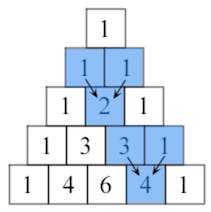
\includegraphics{../img/Pascal triangle half-size.png}

    Você consegue escrever a expressão que gera os itens de uma linha
genérica do triângulo?\\
Experimente começar com um caso particular. Por exemplo, o quarto item
da linha 5 é formado pela soma do terceiro e quarto itens da linha 4.
Podemos conseguir esse efeito somando duas cópias da linha 4, deslocadas
de uma coluna, ...  
$$
\begin{array}{ r | c  c  c  c  c }
   linha \,4             & 1 & 3 & 3 & 1 &    \\ 
   linha \,4\, deslocada &   & 1 & 3 & 3 & 1  \\ \hline
   linha \,5             & 1 & 4 & 6 & 4 & 1  \\ 
\end{array}
$$
    Suponha que a linha 4 esteja representada numa lista \(\mathit{tp}\).\\
Podemos ajustar o comprimento das duas linhas anexando uma lista \([0]\)
nas posições adequadas.\\
A primeira linha da tabela será dada por \(\mathit{tp} + [0]\).\\
A segunda linha da tabela, por sua vez, será dada por
\([0] + \mathit{tp}\).\\
Para ``emparelhar'' essas duas linhas podemos usar a função
\(\mathit{zip}\) e depois somar os itens correspondentes usando um
\(\mathit{for}\).

    \begin{Verbatim}[commandchars=\\\{\}]
{\color{incolor}In [{\color{incolor}40}]:} \PY{k}{def} \PY{n+nf}{triângulo\PYZus{}de\PYZus{}pascal}\PY{p}{(}\PY{n}{n}\PY{p}{)}\PY{p}{:}
             
             \PY{k}{def} \PY{n+nf}{próxima\PYZus{}linha}\PY{p}{(}\PY{n}{tp}\PY{p}{)}\PY{p}{:}
                 \PY{k}{if} \PY{n}{tp}\PY{p}{:}
                     \PY{n}{ptp} \PY{o}{=} \PY{p}{[}\PY{p}{]}
                     \PY{k}{for} \PY{n}{esq}\PY{p}{,} \PY{n+nb}{dir} \PY{o+ow}{in} \PY{n+nb}{zip}\PY{p}{(}\PY{n}{tp} \PY{o}{+} \PY{p}{[}\PY{l+m+mi}{0}\PY{p}{]}\PY{p}{,} \PY{p}{[}\PY{l+m+mi}{0}\PY{p}{]} \PY{o}{+} \PY{n}{tp}\PY{p}{)}\PY{p}{:}
                         \PY{n}{ptp} \PY{o}{+}\PY{o}{=} \PY{p}{[}\PY{n}{esq} \PY{o}{+} \PY{n+nb}{dir}\PY{p}{]}
                     \PY{k}{return} \PY{n}{ptp}
                 \PY{k}{else}\PY{p}{:}
                     \PY{k}{return} \PY{p}{[}\PY{l+m+mi}{1}\PY{p}{]}
         
             \PY{k}{if} \PY{o+ow}{not} \PY{n+nb}{isinstance}\PY{p}{(}\PY{n}{n}\PY{p}{,} \PY{n+nb}{int}\PY{p}{)} \PY{o+ow}{or} \PY{n}{n} \PY{o}{\PYZlt{}} \PY{l+m+mi}{1}\PY{p}{:}
                 \PY{k}{return} \PY{k+kc}{None}
             \PY{k}{else}\PY{p}{:}
                 \PY{n}{tp} \PY{o}{=} \PY{p}{[}\PY{p}{]}
                 \PY{k}{for} \PY{n}{linha} \PY{o+ow}{in} \PY{n+nb}{range}\PY{p}{(}\PY{n}{n}\PY{p}{)}\PY{p}{:}
                     \PY{n}{tp} \PY{o}{=} \PY{n}{próxima\PYZus{}linha}\PY{p}{(}\PY{n}{tp}\PY{p}{)}
                     \PY{n+nb}{print}\PY{p}{(}\PY{n}{tp}\PY{p}{)}
                 
         \PY{n}{triângulo\PYZus{}de\PYZus{}pascal}\PY{p}{(}\PY{l+m+mi}{6}\PY{p}{)}
\end{Verbatim}


    \begin{Verbatim}[commandchars=\\\{\}]
[1]
[1, 1]
[1, 2, 1]
[1, 3, 3, 1]
[1, 4, 6, 4, 1]
[1, 5, 10, 10, 5, 1]

    \end{Verbatim}

    Finalmente, é possível compactar a função \(\mathit{próxima\_linha}\)
usando uma \emph{list comprehension}.

    \begin{Verbatim}[commandchars=\\\{\}]
{\color{incolor}In [{\color{incolor}41}]:} \PY{k}{def} \PY{n+nf}{triângulo\PYZus{}de\PYZus{}pascal}\PY{p}{(}\PY{n}{n}\PY{p}{)}\PY{p}{:}
             
             \PY{k}{def} \PY{n+nf}{próxima\PYZus{}linha}\PY{p}{(}\PY{n}{tp}\PY{p}{)}\PY{p}{:}
                 \PY{k}{if} \PY{n}{tp}\PY{p}{:}
                     \PY{k}{return} \PY{p}{[}\PY{n}{esq} \PY{o}{+} \PY{n+nb}{dir} \PY{k}{for} \PY{n}{esq}\PY{p}{,} \PY{n+nb}{dir} \PY{o+ow}{in} \PY{n+nb}{zip}\PY{p}{(}\PY{n}{tp} \PY{o}{+} \PY{p}{[}\PY{l+m+mi}{0}\PY{p}{]}\PY{p}{,} \PY{p}{[}\PY{l+m+mi}{0}\PY{p}{]} \PY{o}{+} \PY{n}{tp}\PY{p}{)}\PY{p}{]}
                 \PY{k}{else}\PY{p}{:}
                     \PY{k}{return} \PY{p}{[}\PY{l+m+mi}{1}\PY{p}{]}
         
             \PY{k}{if} \PY{o+ow}{not} \PY{n+nb}{isinstance}\PY{p}{(}\PY{n}{n}\PY{p}{,} \PY{n+nb}{int}\PY{p}{)} \PY{o+ow}{or} \PY{n}{n} \PY{o}{\PYZlt{}} \PY{l+m+mi}{1}\PY{p}{:}
                 \PY{k}{return} \PY{k+kc}{None}
             \PY{k}{else}\PY{p}{:}
                 \PY{n}{tp} \PY{o}{=} \PY{p}{[}\PY{p}{]}
                 \PY{k}{for} \PY{n}{linha} \PY{o+ow}{in} \PY{n+nb}{range}\PY{p}{(}\PY{n}{n}\PY{p}{)}\PY{p}{:}
                     \PY{n}{tp} \PY{o}{=} \PY{n}{próxima\PYZus{}linha}\PY{p}{(}\PY{n}{tp}\PY{p}{)}
                     \PY{n+nb}{print}\PY{p}{(}\PY{n}{tp}\PY{p}{)}
                 
         \PY{n}{triângulo\PYZus{}de\PYZus{}pascal}\PY{p}{(}\PY{l+m+mi}{6}\PY{p}{)}
\end{Verbatim}


    \begin{Verbatim}[commandchars=\\\{\}]
[1]
[1, 1]
[1, 2, 1]
[1, 3, 3, 1]
[1, 4, 6, 4, 1]
[1, 5, 10, 10, 5, 1]

    \end{Verbatim}


    % Add a bibliography block to the postdoc
    
    
    
    \end{document}
